% The Stage 2 report: the parts of the three members, assembled (plan DR-15). Section numbers follow the
% list of assignment section 7.1, where the cover is number 1.
%   cover, 2, 4, Search parts of 5 and 7 ......... Daniel Perdomo (search_part.tex, DP-13)
%   3, Ingestion and Control of 5, coordination of 6, 8 ... Carlos Falcon (coordination_part.tex, CF-14)
%   Indexing of 5, storage of 6, Indexing of 7, consolidation of 7 ... Daniel Rodriguez (indexing_part.tex, DR-15)
%
% Build from docs/report/:  pdflatex report.tex && pdflatex report.tex   (twice, for the contents and references)
% The figures of Indexing come from: python3 benchmarks/plot.py --format pdf --out docs/report/figures
% \pending{...} marks what still depends on the measures: it must not reach the final PDF.
\documentclass[11pt,a4paper]{article}

\usepackage[utf8]{inputenc}
\usepackage[T1]{fontenc}
\usepackage{lmodern}
\usepackage{microtype}
\usepackage[margin=2.4cm,headheight=14pt]{geometry}
\usepackage{graphicx}
\usepackage{booktabs}
\usepackage{tabularx}
\usepackage{array}
\usepackage{enumitem}
\usepackage{float}
\usepackage{xcolor}
\usepackage{listings}
\usepackage{fancyhdr}
\usepackage{titlesec}
\usepackage{tikz}
\usetikzlibrary{arrows.meta,positioning,fit,backgrounds,calc,shadows}
\usepackage[hidelinks]{hyperref}

\definecolor{accent}{HTML}{2a78d6}
\definecolor{ink}{HTML}{0b0b0b}
\definecolor{muted}{HTML}{52514e}
\definecolor{codebg}{HTML}{f6f6f4}
\definecolor{rule}{HTML}{d8d7d2}
\definecolor{pendingink}{HTML}{b3261e}

\hypersetup{colorlinks=true,linkcolor=accent,urlcolor=accent,citecolor=accent}
\hypersetup{
  pdftitle={Search Engine Project. Stage 2: Service-Oriented Architecture},
  pdfauthor={Daniel Rodríguez Alonso (79072763M), Daniel Perdomo Medina (54173402F), Carlos Falcón Brito (54149163X)},
  pdfsubject={Big Data, ULPGC. Group BigData-Ulpgc},
}

\titleformat{\section}{\Large\bfseries\color{ink}}{\thesection.}{0.6em}{}
\titleformat{\subsection}{\large\bfseries\color{ink}}{\thesubsection}{0.6em}{}
\titlespacing*{\section}{0pt}{1.6em}{0.7em}
\titlespacing*{\subsection}{0pt}{1.2em}{0.5em}

\pagestyle{fancy}
\fancyhf{}
\fancyhead[L]{\small\color{muted}Stage 2 $\cdot$ Service-oriented architecture}
\fancyhead[R]{\small\color{muted}Big Data $\cdot$ ULPGC}
\fancyfoot[C]{\small\thepage}
\renewcommand{\headrulewidth}{0.4pt}

\setlist{itemsep=2pt,topsep=4pt}
\setlength{\parskip}{0.45em}
\setlength{\parindent}{0pt}
\setlength{\emergencystretch}{3em}
\renewcommand{\arraystretch}{1.25}

\lstset{language={}, basicstyle=\ttfamily\footnotesize, backgroundcolor=\color{codebg}, frame=single,
  rulecolor=\color{rule}, framesep=4pt, xleftmargin=6pt, xrightmargin=6pt, breaklines=true,
  columns=fullflexible, keepspaces=true, showstringspaces=false, aboveskip=8pt, belowskip=8pt}

\newcolumntype{L}[1]{>{\raggedright\arraybackslash}p{#1}}
\newcommand{\code}[1]{\texttt{#1}}
\newcommand{\pending}[1]{\par\medskip{\color{pendingink}\textbf{[PENDING]} #1}\par\medskip}


% The parts of sections 5, 6 and 7 are written as sections of their own ("Microservice implementation: Indexing").
% Inside the final report each becomes a subsection of its section, titled with what follows the colon.
\setcounter{secnumdepth}{3}
\makeatletter
\let\origsubsection\subsection
\let\origsubsubsection\subsubsection
\def\partsection@title#1: #2#3\@nil{\MakeUppercase{#2}#3}
\newcommand{\partsection}[1]{\origsubsection{\partsection@title#1\@nil}}
\newenvironment{parts}{\let\section\partsection\let\subsection\origsubsubsection\let\subsubsection\paragraph}{}
\makeatother

\begin{document}

\begin{titlepage}
\thispagestyle{empty}
\vspace*{2.5cm}
{\color{accent}\rule{\linewidth}{1.2pt}}\\[0.8cm]
{\Huge\bfseries Search Engine Project\par}
\vspace{0.4cm}
{\LARGE Stage 2: Service-Oriented Architecture\par}
\vspace{0.6cm}
{\color{accent}\rule{\linewidth}{1.2pt}}
\vspace{2cm}

\begin{tabular}{@{}>{\bfseries}L{3.4cm}L{10.5cm}@{}}
Course & Big Data $\cdot$ Grado en Ciencia e Ingeniería de Datos $\cdot$ Universidad de Las Palmas de Gran Canaria \\
Academic year & 2026/2027 \\
Group name & BigData-Ulpgc \\
Members & Daniel Rodríguez Alonso --- 79072763M \\
 & Daniel Perdomo Medina --- 54173402F \\
 & Carlos Falcón Brito --- 54149163X \\
Repository & \url{https://github.com/BigData-Ulpgc/stage_2} \\
\end{tabular}
\vfill
\end{titlepage}

\tableofcontents
\clearpage

\setcounter{section}{1}
\section{Introduction and objectives}
\label{sec:intro}

Stage 1 built and measured the data layer of a search engine over the books of Project Gutenberg: a
datalake, an inverted index and a metadata store. Stage 2 turns that data layer into a system of
cooperating services that keeps working while books are being added and users are searching, all on a
single machine.

The system has four kinds of process. \textbf{Ingestion} downloads books and stores them in the datalake.
\textbf{Indexing} adds complete books to the index and publishes new versions of it. \textbf{Search}
answers the front-end. The \textbf{Control Module} decides what has to be done and when, without doing
any of the work itself. They coordinate through Hazelcast and share their results through the datalake and
MongoDB. A front-end only sees one public API, behind nginx.

The objectives of the stage, and how the system meets them, are:

\begin{itemize}
  \item \textbf{Clear contracts.} Every HTTP endpoint is specified in OpenAPI and classified as
        front-end, internal or operational, and the interactions that are not HTTP have their own
        contracts (Section~\ref{sec:api}).
  \item \textbf{Correct behaviour under concurrency.} A book is only indexed once complete, each book
        is processed by one worker at a time, and a search never sees a partially published version.
  \item \textbf{Survival of failures.} A worker that dies loses its lease and its book returns to the
        queue. If Hazelcast loses its state, the Control rebuilds it from what is persistent. If a Search
        replica dies, nginx sends the request to another one.
  \item \textbf{Reproducible deployment.} One command starts every process with fixed resource limits,
        and the number of replicas and threads of each service is configurable
        (Section~\ref{sec:deployment}).
  \item \textbf{Evidence.} The APIs are checked automatically against the running system, and the
        benchmarks identify what limits performance on one machine, keeping client concurrency, threads
        and replicas apart (Section~\ref{sec:benchmarks}).
\end{itemize}

Everything runs on one host by design: replicas and threads share its CPU, memory and disk. What these
measures say about one machine does not establish how the system will scale on the Stage 3 cluster.

\section{System architecture}
\label{sec:architecture}

The search engine of Stage 1 becomes four cooperating services, each a Maven module that builds an executable
jar and a Docker image: \textbf{Ingestion} downloads books into the datalake, \textbf{Indexing} turns them into
the inverted index and the metadata in MongoDB, \textbf{Search} answers the queries of the front-end, and the
\textbf{Control Module} feeds and supervises the pipeline. They never call each other to hand over work: they
share it through a \textbf{Hazelcast} cluster, which holds the state of every book and the queues of work. Only two
calls go over HTTP between services: the Control asks Indexing to publish, and the administrators call the
internal APIs directly.

\subsection{Coordination mechanism}

The design combines two of the mechanisms the assignment allows:

\begin{itemize}
  \item \textbf{A shared-memory region:} the Hazelcast cluster (two members, version 5.7.0). It is the only place
    where the services meet. It holds the state of every book (\code{book-state}), the two queues of work
    (\code{ingest-queue} and \code{index-queue}), the lock of the single index writer (\code{index-writer}), the
    event of each new version of the index (\code{index-events}) and a marker that tells whether the cluster still
    has its state (\code{coordination-meta}). All access goes through one library in \code{common}
    (\code{Coordination}), so no service builds a key, a value or a transaction by hand.
  \item \textbf{A scheduler:} the Control Module. It seeds the books, reviews the leases every
    \code{LEASE\_CHECK\_SECONDS} and decides when a new version of the index is published. It is not in the path of
    any book: the workers take their work from the queues, and keep doing so while the Control is down.
\end{itemize}

There is no message broker. Hazelcast's queues have no acknowledgements, so a book taken by a worker that dies would
be lost from the queue; the leases in \code{book-state} recover it (Section~\ref{sec:ownership}). The persistent
truth is not in Hazelcast but in the datalake and MongoDB: Hazelcast only says who does what, and a book changes state
only after its evidence is on disk. If the whole cluster is lost, the Control rebuilds it from that evidence.

\subsection{Deployment on one host}

Every process runs on one machine, started by Docker Compose from \code{docker-compose.yml} and \code{.env}
(Figure~\ref{fig:deployment}). Each container has fixed \code{cpus} and \code{mem\_limit}, so the experiments are
reproducible. The only entry from outside is nginx: it is the \textbf{front-end API boundary}, and everything to its
right in the figure is internal.

\begin{figure}[H]
\centering
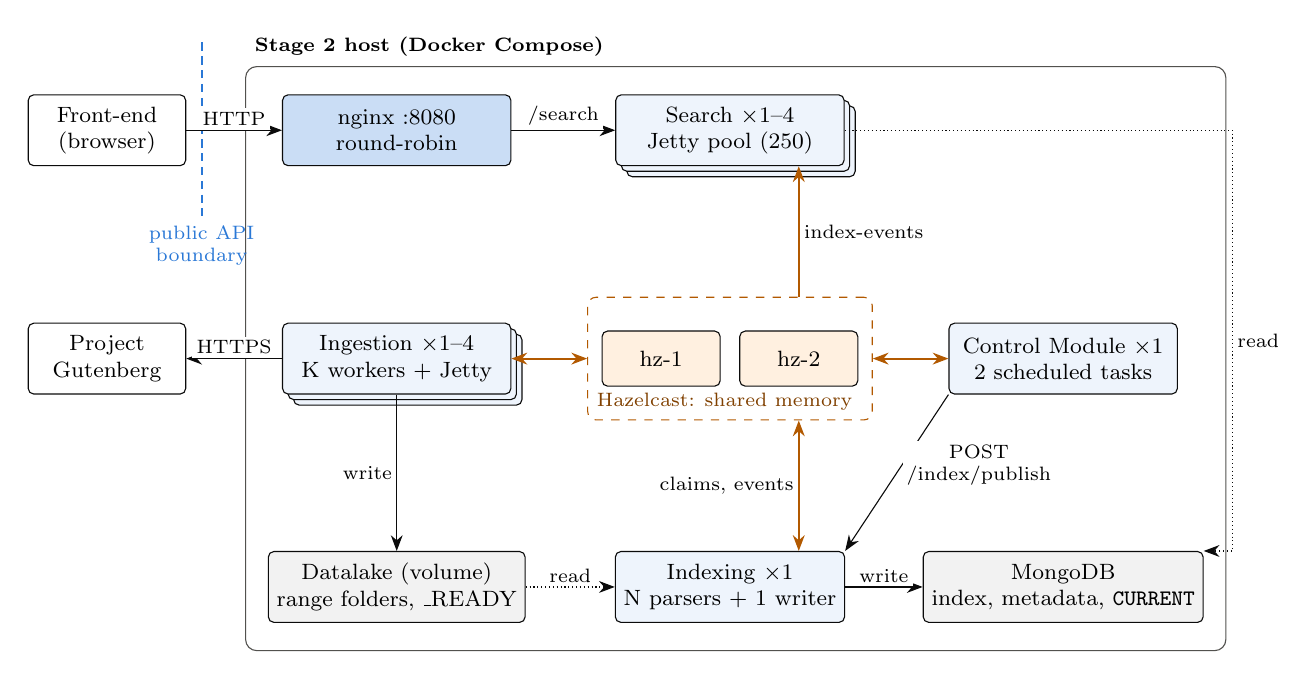
\begin{tikzpicture}[
    font=\footnotesize, x=0.92cm,
    box/.style={draw=ink, rounded corners=2pt, align=center, fill=white, minimum height=9mm, inner sep=3pt},
    svc/.style={box, fill=accent!8, minimum width=29mm},
    rep/.style={svc, double copy shadow={shadow xshift=2pt, shadow yshift=-2pt}},
    store/.style={box, fill=black!5, minimum width=29mm},
    hz/.style={box, fill=orange!12, minimum width=15mm, minimum height=7mm},
    arr/.style={-{Stealth[length=2mm]}, draw=ink},
    hzl/.style={{Stealth[length=2mm]}-{Stealth[length=2mm]}, draw=orange!70!black, thick},
    lab/.style={font=\scriptsize, fill=white, inner sep=1.5pt, align=center},
  ]
  % Hazelcast in the middle: every service meets there
  \node[hz] (hz1) at (-0.35,0) {hz-1};
  \node[hz] (hz2) at (1.55,0) {hz-2};
  \node[draw=orange!70!black, dashed, rounded corners=3pt, fit=(hz1)(hz2), inner xsep=5pt, inner ysep=12pt] (hz) {};
  \node[font=\scriptsize, text=orange!50!black, anchor=south west] at (hz.south west) {Hazelcast: shared memory};

  % Services around it
  \node[rep] (search) at (0.6,2.9) {Search $\times$1--4\\Jetty pool (250)};
  \node[rep] (ingestion) at (-4.0,0) {Ingestion $\times$1--4\\K workers + Jetty};
  \node[svc] (control) at (5.2,0) {Control Module $\times$1\\2 scheduled tasks};
  \node[svc] (indexing) at (0.6,-2.9) {Indexing $\times$1\\N parsers + 1 writer};
  \node[svc, fill=accent!25] (nginx) at (-4.0,2.9) {nginx :8080\\round-robin};

  % Shared storage
  \node[store] (datalake) at (-4.0,-2.9) {Datalake (volume)\\range folders, \_READY};
  \node[store] (mongo) at (5.2,-2.9) {MongoDB\\index, metadata, \code{CURRENT}};

  % Outside the host
  \node[box, minimum width=20mm] (client) at (-8.0,2.9) {Front-end\\(browser)};
  \node[box, minimum width=20mm] (gutenberg) at (-8.0,0) {Project\\Gutenberg};

  % The host
  \begin{scope}[on background layer]
    \node[draw=muted, rounded corners=4pt, fit=(nginx)(search)(control)(mongo)(datalake), inner xsep=8pt, inner ysep=10pt]
      (host) {};
  \end{scope}
  \node[font=\scriptsize\bfseries, anchor=south west] at (host.north west) {Stage 2 host (Docker Compose)};
  \draw[densely dashed, accent, thick] ($(host.north west)+(-0.6,0.3)$) -- ($(host.north west)+(-0.6,-1.9)$)
    node[below, font=\scriptsize, text=accent, align=center] {public API\\boundary};

  % Hazelcast clients
  \draw[hzl] (ingestion) -- (hz);
  \draw[hzl] (control) -- (hz);
  \draw[hzl] (indexing.north -| hz2) -- node[lab, left] {claims, events} (hz.south -| hz2);
  \draw[-{Stealth[length=2mm]}, draw=orange!70!black, thick] (hz.north -| hz2) -- node[lab, right] {index-events} (search.south -| hz2);

  % HTTP
  \draw[arr] (client) -- node[lab, above] {HTTP} (nginx);
  \draw[arr] (nginx) -- node[lab, above] {/search} (search);
  \draw[arr] (control.south west) -- node[lab, right, pos=0.45] {POST\\/index/publish} (indexing.north east);
  \draw[arr] (ingestion) -- node[lab, above] {HTTPS} (gutenberg);

  % Storage
  \draw[arr] (ingestion) -- node[lab, left] {write} (datalake);
  \draw[arr, densely dotted] (datalake) -- node[lab, above] {read} (indexing);
  \draw[arr] (indexing) -- node[lab, above] {write} (mongo);
  \draw[arr, densely dotted] (search.east) -| node[lab, pos=0.75, right] {read} ($(mongo.north east)+(0.4,0)$)
    -- (mongo.north east);
\end{tikzpicture}
\caption{The deployment on the single Stage 2 host. Only nginx is reachable from other machines; the Control
(\code{127.0.0.1:7000}), Hazelcast and MongoDB are published on the loopback interface for the administrator and
the tests. Orange: Hazelcast clients (a client reaches both members). Dotted: read-only access to shared storage.
A shadow marks a service that can run several replicas.}
\label{fig:deployment}
\end{figure}

\textbf{Shared storage.} Two stores are shared, each with a single writer:
\begin{itemize}
  \item The \textbf{datalake} is a bind-mounted folder. Ingestion writes it; Indexing and the Control only read it
    (read-only mounts). Books are grouped in folders of 1,000 ids (\code{01000-01999}), each with
    \code{<id>.header.txt}, \code{<id>.body.txt} and, written last, \code{<id>.\_READY}: a book exists only with
    its marker (Section~\ref{sec:readiness}).
  \item \textbf{MongoDB} holds the inverted index, the metadata of the books, the log of indexed books
    (\code{index\_log}), the books of each published version (\code{index\_books}) and the pointer \code{CURRENT}.
    Indexing writes; Search reads; the Control reads it only to recover.
\end{itemize}

\textbf{Replicas and threads.} Table~\ref{tab:replicas} separates the three kinds of concurrency of the system:
process replicas, threads inside a process, and client concurrency, which only exists in front of Search.

\begin{table}[H]
\centering\small
\begin{tabularx}{\linewidth}{@{}L{2.2cm}L{1.8cm}L{3.9cm}X@{}}
\toprule
\textbf{Process} & \textbf{Replicas} & \textbf{Threads} & \textbf{How work is shared} \\
\midrule
Ingestion & 1--4 (\code{-{}-scale}) & \code{INGESTION\_WORKERS} (4) workers; Jetty pool & Every worker of every replica
  claims from the same \code{ingest-queue}: Hazelcast distributes the books, and nobody knows the address of a replica \\
Indexing & 1--2 & \code{INDEXING\_THREADS} (4) parsers; one writer & Only the replica that holds \code{index-writer}
  claims from \code{index-queue} and writes the index; another one would wait as a standby \\
Search & 1--4 (\code{-{}-scale}) & Jetty pool, \code{SEARCH\_HTTP\_THREADS} (250) & nginx sends each request to the
  next replica (round-robin); each one reads an immutable snapshot \\
Control & 1 & 2 scheduled tasks; Jetty pool & Not in the path of a book: lease check and publication \\
Hazelcast & 2 members & managed by Hazelcast & 271 partitions spread over both, each with one backup on the other \\
MongoDB & 1 & managed by MongoDB & Shared by Indexing (writes) and every Search replica (reads) \\
\bottomrule
\end{tabularx}
\caption{Replicas and threads of each process. The Jetty pool of every service is explicit: Javalin 6.1.3 creates a
\code{QueuedThreadPool} with at most 250 threads, at least 8 and 60~s of idle time, and
\code{<SERVICE>\_HTTP\_THREADS} changes the maximum.}
\label{tab:replicas}
\end{table}

\subsection{The life of a book}

\code{book-state} keeps one entry per book with its state, its owner and its lease, and the transitions are the
only way to change it (Figure~\ref{fig:states}). Each transition is a compare-and-set, \code{replace(id, expected,
next)}, which succeeds only if nobody changed the entry since it was read; one that also moves the id to or from a
queue runs in one Hazelcast transaction with that queue operation, so a crash never does one without the other.

\begin{figure}[H]
\centering
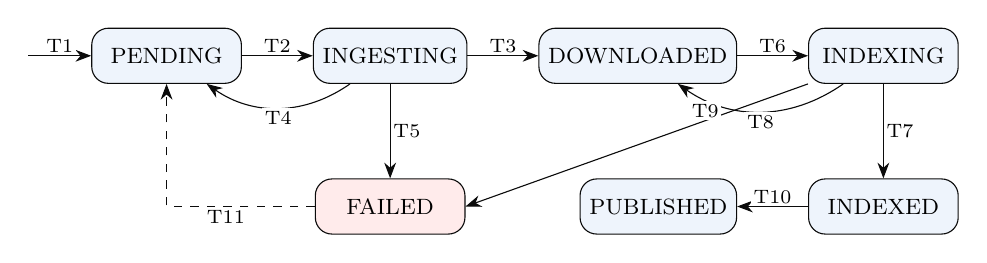
\begin{tikzpicture}[
    font=\footnotesize, node distance=6mm and 9mm,
    st/.style={draw=ink, rounded corners=6pt, fill=accent!8, minimum width=19mm, minimum height=7mm},
    arr/.style={-{Stealth[length=2mm]}, draw=ink},
    lab/.style={font=\scriptsize, fill=white, inner sep=1pt},
  ]
  \node[st] (pending) {PENDING};
  \node[st, right=of pending] (ingesting) {INGESTING};
  \node[st, right=of ingesting] (downloaded) {DOWNLOADED};
  \node[st, right=of downloaded] (indexing) {INDEXING};
  \node[st, below=12mm of indexing] (indexed) {INDEXED};
  \node[st, left=of indexed] (published) {PUBLISHED};
  \node[st, fill=red!8, below=12mm of ingesting] (failed) {FAILED};

  \draw[arr] ($(pending.west)+(-8mm,0)$) -- node[lab, above] {T1} (pending);
  \draw[arr] (pending) -- node[lab, above] {T2} (ingesting);
  \draw[arr] (ingesting) -- node[lab, above] {T3} (downloaded);
  \draw[arr] (downloaded) -- node[lab, above] {T6} (indexing);
  \draw[arr] (indexing) -- node[lab, right] {T7} (indexed);
  \draw[arr] (indexed) -- node[lab, above] {T10} (published);
  \draw[arr, bend left=35] (ingesting) to node[lab, below] {T4} (pending);
  \draw[arr, bend left=35] (indexing) to node[lab, below] {T8} (downloaded);
  \draw[arr] (ingesting) -- node[lab, right] {T5} (failed);
  \draw[arr] (indexing.south west) -- node[lab, pos=0.3, above] {T9} (failed.east);
  \draw[arr, dashed] (failed.west) -| node[lab, pos=0.3, below] {T11} (pending.south);
\end{tikzpicture}
\caption{The states of a book (coordination contract §4). T2/T6 claim the book with a lease; T3/T7 complete the
stage once its evidence is persistent; T4/T8 requeue it after a transient failure or an expired lease; T5/T9 send it
to \code{FAILED} after a permanent error or the last attempt; T10 marks it visible; T11 is
\code{POST /control/retry-failed}. The recovery (row R, Section~\ref{sec:recovery}) may also create an entry directly
as \code{DOWNLOADED}, \code{INDEXED} or \code{PUBLISHED}.}
\label{fig:states}
\end{figure}

Figure~\ref{fig:sequence} follows one book through the whole system. The order matters: each step writes its
evidence before the state that announces it, so a crash between both leaves a book that is either redone or
recovered, never one that is announced but missing.

\begin{figure}[H]
\centering
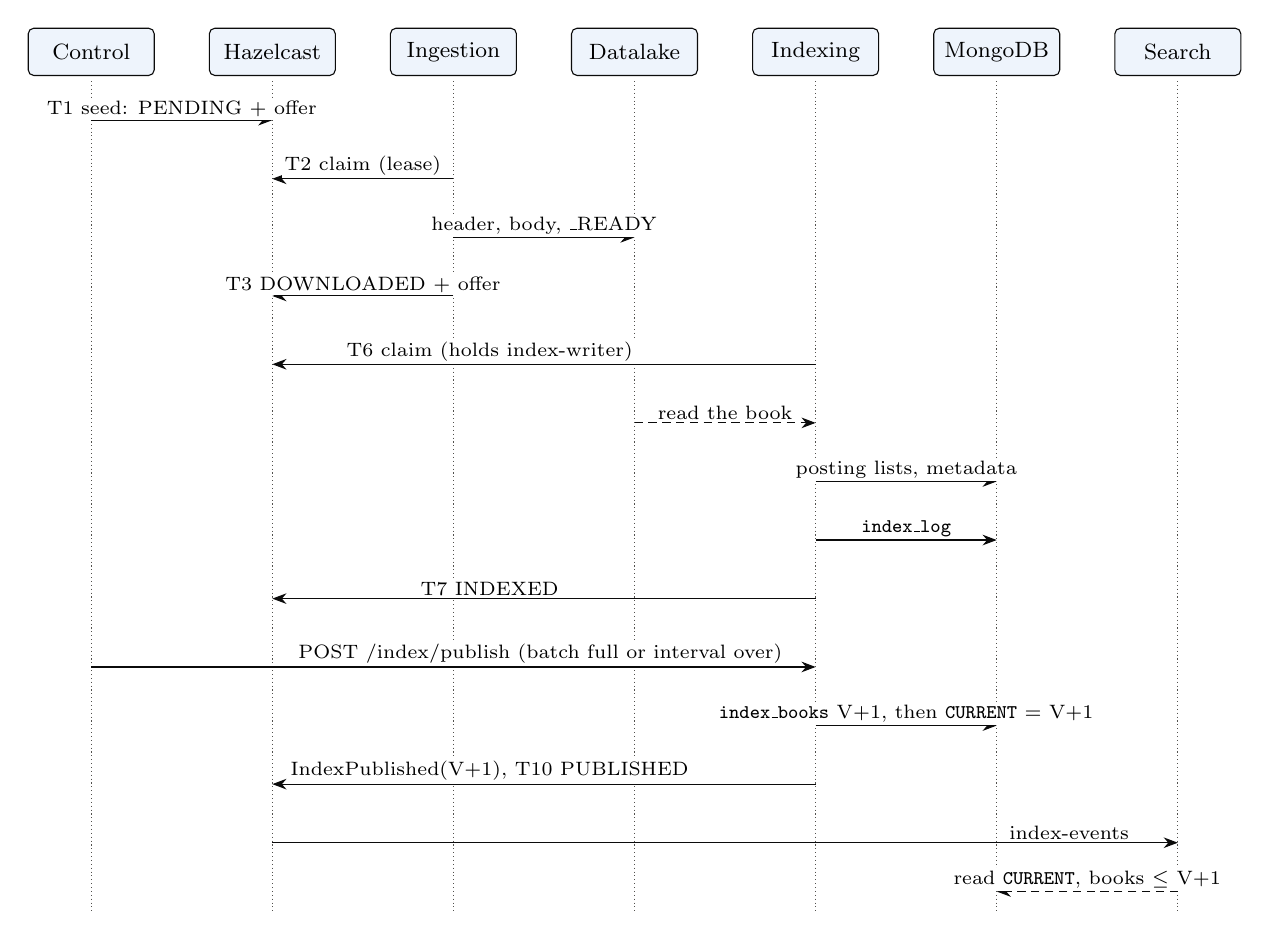
\begin{tikzpicture}[
    font=\scriptsize, x=1cm, y=-0.62cm,
    head/.style={draw=ink, rounded corners=2pt, fill=accent!8, minimum width=16mm, minimum height=6mm, font=\footnotesize},
    msg/.style={-{Stealth[length=1.8mm]}, draw=ink},
    note/.style={font=\scriptsize, fill=white, inner sep=1pt},
  ]
  \foreach \x/\n/\t in {0/C/Control, 2.3/H/Hazelcast, 4.6/I/Ingestion, 6.9/D/Datalake, 9.2/X/Indexing,
                         11.5/M/MongoDB, 13.8/S/Search} {
    \node[head] (\n) at (\x,0) {\t};
    \draw[muted, densely dotted] (\x,0.6) -- (\x,17.6);
  }
  \draw[msg] (0,1.4) -- node[note, above] {T1 seed: PENDING + offer} (2.3,1.4);
  \draw[msg] (4.6,2.6) -- node[note, above] {T2 claim (lease)} (2.3,2.6);
  \draw[msg] (4.6,3.8) -- node[note, above] {header, body, \_READY} (6.9,3.8);
  \draw[msg] (4.6,5.0) -- node[note, above] {T3 DOWNLOADED + offer} (2.3,5.0);
  \draw[msg] (9.2,6.4) -- node[note, above, pos=0.6] {T6 claim (holds index-writer)} (2.3,6.4);
  \draw[msg, densely dashed] (6.9,7.6) -- node[note, above] {read the book} (9.2,7.6);
  \draw[msg] (9.2,8.8) -- node[note, above] {posting lists, metadata} (11.5,8.8);
  \draw[msg] (9.2,10.0) -- node[note, above] {\code{index\_log}} (11.5,10.0);
  \draw[msg] (9.2,11.2) -- node[note, above, pos=0.6] {T7 INDEXED} (2.3,11.2);
  \draw[msg] (0,12.6) -- node[note, above, pos=0.62] {POST /index/publish (batch full or interval over)} (9.2,12.6);
  \draw[msg] (9.2,13.8) -- node[note, above] {\code{index\_books} V+1, then \code{CURRENT} = V+1} (11.5,13.8);
  \draw[msg] (9.2,15.0) -- node[note, above, pos=0.6] {IndexPublished(V+1), T10 PUBLISHED} (2.3,15.0);
  \draw[msg] (2.3,16.2) -- node[note, above, pos=0.88] {index-events} (13.8,16.2);
  \draw[msg, densely dashed] (13.8,17.2) -- node[note, above] {read \code{CURRENT}, books $\le$ V+1} (11.5,17.2);
\end{tikzpicture}
\caption{The flow of one book. Dashed: reads. Every arrow towards Hazelcast is a transition of
Figure~\ref{fig:states}; each one comes after the evidence it announces (\code{\_READY}, \code{index\_log},
\code{CURRENT}).}
\label{fig:sequence}
\end{figure}

\begin{enumerate}
  \item \textbf{Seed.} \code{POST /control/jobs} (or \code{CONTROL\_SEED\_FILE}) puts every unknown id as
    \code{PENDING} and offers it to \code{ingest-queue}. A known id is left as it is, so seeding twice duplicates
    nothing.
  \item \textbf{Ingestion.} A worker claims the id: one transaction polls the queue and writes \code{INGESTING} with
    its name and a lease of \code{LEASE\_SECONDS}. It downloads the book, splits header and body, writes both files
    and then the \code{\_READY} marker, and completes: \code{DOWNLOADED} and an offer to \code{index-queue}, again in
    one transaction.
  \item \textbf{Indexing.} The replica that holds \code{index-writer} claims from \code{index-queue}, parses and
    tokenizes the books in parallel, writes the posting lists and the metadata to MongoDB in batches, records each book
    in \code{index\_log} and marks it \code{INDEXED}. The book is in the index, but Search does not show it yet.
  \item \textbf{Publication.} When \code{PUBLISH\_BATCH} books (100) are \code{INDEXED}, or \code{PUBLISH\_INTERVAL\_S}
    (30~s) have passed with at least one, the Control calls \code{POST /index/publish}. Indexing records the new books in
    \code{index\_books} with version V+1 and moves \code{CURRENT} to V+1 in one atomic update; the index itself is not
    copied. Right after answering, it announces \code{IndexPublished} and marks the books \code{PUBLISHED}.
  \item \textbf{Reload.} Every Search replica receives the event, reads \code{CURRENT} and the books up to it, and
    swaps its immutable snapshot. A lost event is covered by its periodic check of \code{CURRENT}.
\end{enumerate}

\textbf{Operational endpoints.} Every service answers \code{GET /status} without touching Hazelcast or MongoDB, so a
healthcheck never fails because a dependency is down; the Docker healthchecks and \code{depends\_on} use it. The
Control adds \code{GET /control/status} with the books per state and the size of each queue, the observation point of
the whole pipeline (Section~\ref{sec:api}).

\section{API design and contracts}
\label{sec:api}

The full specifications are in the repository, one OpenAPI document per service because every service has
a \code{GET /status}: \code{api/openapi.yaml} (Search), \code{api/indexing-openapi.yaml},
\code{api/ingestion-openapi.yaml} and \code{api/control-openapi.yaml}. The inventory of every endpoint is
\code{api/endpoints.md}. This section summarises them.

\subsection{Front-end use cases}

A front-end needs three things, and it reaches them only through nginx on port 8080:

\begin{itemize}
  \item Search books by keywords, optionally by author, language and year, one page at a time.
  \item Show the details of one book.
  \item Offer the available filters: the languages and the range of years of the published index.
\end{itemize}

\begin{table}[H]
\centering\small
\begin{tabularx}{\linewidth}{@{}L{4.6cm}L{1.6cm}X@{}}
\toprule
\textbf{Endpoint} & \textbf{Provider} & \textbf{Purpose} \\
\midrule
\code{GET /search} & Search & Keyword search (AND) with filters and pagination \\
\code{GET /books/\{book\_id\}} & Search & Metadata of one published book \\
\code{GET /search/filters} & Search & Languages and year range of the published index \\
\bottomrule
\end{tabularx}
\caption{Front-end inventory. All are read-only, so they are safe to retry.}
\end{table}

\subsection{Internal and operational interfaces}

These are consumed by another service or by an operator, never by the front-end. Only the Control Module
is published on the host, on \code{127.0.0.1}; the others are reached by name inside the Docker network.

\begin{table}[H]
\centering\small
\begin{tabularx}{\linewidth}{@{}L{4.9cm}L{2.4cm}X@{}}
\toprule
\textbf{Endpoint} & \textbf{Consumer} & \textbf{Completion} \\
\midrule
\code{POST /ingest/\{book\_id\}} & operators, validation & Done: the book is stored, or was already available \\
\code{GET /ingest/status/\{book\_id\}} & operators, validation & Done (read-only) \\
\code{GET /ingest/list} & operators, validation & Done (read-only) \\
\code{POST /index/update/\{book\_id\}} & operators, validation & Done: indexed, but not visible until published \\
\code{POST /index/publish} & Control Module & Done: \code{CURRENT} points to the returned version \\
\code{POST /index/rebuild} & operators & Accepted: continues in the background \\
\code{GET /index/status} & Control, operators & Done (read-only) \\
\code{POST /control/jobs} & operators, benchmarks & Accepted (202): follow it with \code{/control/status} \\
\code{GET /control/status} & operators, benchmarks & Done (read-only) \\
\code{GET /control/tasks/\{book\_id\}} & operators, validation & Done (read-only) \\
\code{POST /control/retry-failed} & operators & Accepted: the books are back in their queue \\
\midrule
\code{GET /status} (every service) & Docker healthcheck, operators & Done. Liveness only: it does not depend on MongoDB or Hazelcast \\
\bottomrule
\end{tabularx}
\caption{Internal inventory, and the operational endpoint in the last row.}
\end{table}

\subsection{Parameters, pagination and errors}

\code{GET /search} requires \code{q}, tokenised with the same \code{Tokenizer} as Indexing, so a query made
only of stopwords has no terms and is rejected. \code{author} matches part of the name, ignoring case;
\code{language} is an ISO 639-1 code; and \code{year} has four digits. Filters combine with AND.

Pagination uses \code{offset} (default 0) and \code{limit} (default 20, at most 100). \code{total} counts every
match, not only the page, and a valid search without matches answers 200 with an empty list. Results are
ordered by ascending \code{book\_id}, behind a \code{ResultRanking} interface that lets the order change
without touching the search. A ranking by relevance would also need term frequencies, which the index does
not store.

Every response of Search carries \code{index\_version}, the one version it was computed from. All services
share one error format:

\begin{lstlisting}
{"error": {"code": "INVALID_PARAMETER", "message": "limit must be ...", "field": "limit"}}
\end{lstlisting}

\begin{table}[H]
\centering\small
\begin{tabularx}{\linewidth}{@{}L{1.2cm}L{5.4cm}X@{}}
\toprule
\textbf{Status} & \textbf{Code} & \textbf{Meaning} \\
\midrule
400 & \code{MISSING\_PARAMETER}, \code{INVALID\_PARAMETER} & The request is wrong; \code{field} says where \\
404 & \code{NOT\_FOUND} & Unknown book, or a route that does not exist \\
503 & \code{INDEX\_NOT\_READY} & Nothing has been published yet \\
503 & \code{STORAGE\_UNAVAILABLE} & MongoDB does not answer; retry later \\
503 & \code{COORDINATION\_UNAVAILABLE} & The Control has no connection to Hazelcast \\
500 & \code{INTERNAL\_ERROR} & Our bug: the details go to the log, not to the client \\
\bottomrule
\end{tabularx}
\caption{Main errors. Each specification lists those of its service.}
\end{table}

\subsection{Contracts that are not HTTP}

Most of the work between services does not use HTTP:

\begin{itemize}
  \item \textbf{Coordination} (\code{api/contracts/coordination.md}): the Hazelcast map \code{book-state},
        the queues \code{ingest-queue} and \code{index-queue}, the topic \code{index-events} with the
        \code{IndexPublished} event, the lock of the index writer, leases and the transitions of a book.
  \item \textbf{Datalake readiness} (\code{api/contracts/datalake-readiness.md}): ranges of folders and the
        \code{<id>.\_READY} marker, written last, which says a book is complete.
  \item \textbf{Publication in MongoDB:} \code{index\_books}, \code{index\_meta} (\code{CURRENT}) and
        \code{index\_publications}. Switching \code{CURRENT} changes one document, so a new version appears
        all at once. The index itself is not copied, because the entries of a written book never change.
\end{itemize}

\pending{Link the contract of the publication when \code{api/contracts/index-publication.md} exists (plan,
owner Daniel Rodríguez). Today the inventory cites the plan, which is not in the repository.}

\subsection{Validation evidence}

The APIs can be checked without a front-end at three levels, all with their expected results:

\begin{itemize}
  \item \code{scripts/validate-api.sh}: every check with one command against the running system, ending
        with exit code 1 if any fails. On the 15 books of the sample dataset it gives 64 correct, 0 failed and
        0 skipped, both with the books loaded directly and with the same books processed by the complete
        flow (Control, Ingestion, Indexing and publication).
  \item \code{StackValidationTest}: the same contract in JUnit, also checking the shape of the JSON.
  \item \code{http/*.http}: examples to run by hand, documented in \code{http/README.md}.
\end{itemize}

They cover keyword search, each filter alone and combined, valid searches without results, invalid parameters,
pagination, the internal endpoints, and the read-only mounts of the datalake. A check only reports
\textit{skipped} for an endpoint that answers 501; a route that disappears is a failure. The expected answers
were compared with the original texts, so they are not a copy of what the API returns. The load tests refuse
to measure if this validation fails.


\section{Microservice implementation}
\label{sec:implementation}
\begin{parts}
\section{Microservice implementation: Ingestion and Control Module}
\label{sec:ingestion-control}

Both are written in Java 17 with Javalin 6.1.3 and Gson, like the rest, and share \code{common}: the HTTP server
with its error format (\code{ServiceServer}), the configuration from the environment (\code{Env}), the range datalake
and the coordination library. Ingestion implements \code{api/ingestion-openapi.yaml} and the Control
\code{api/control-openapi.yaml}; both are checked against their specification by tests (\code{OpenApiContractTest})
and by \code{scripts/validate-api.sh} on the running stack.

\subsection{Ingestion Service}

\begin{table}[H]
\centering\small
\begin{tabularx}{\linewidth}{@{}L{4.1cm}X@{}}
\toprule
\textbf{Class} & \textbf{Responsibility} \\
\midrule
\code{IngestionApi} & \code{POST /ingest/\{id\}}, \code{GET /ingest/status/\{id\}}, \code{GET /ingest/list}, \code{GET /status} \\
\code{IngestionService} & One ingestion, without HTTP: locate, fetch, split, save. The API and the workers run this same code \\
\code{GutenbergClient}, \code{LocalFileSource} & The two sources (\code{INGESTION\_SOURCE}): the download, or \code{pg<id>.txt} files of a folder \\
\code{BookSplitter} & Header and body between the \code{*** START} and \code{*** END} markers, migrated from Stage 1 \\
\code{IngestionWorkers}, \code{IngestionWorker} & The \code{INGESTION\_WORKERS} consumers of \code{ingest-queue} \\
\code{Throttle} & One pause for the whole replica after a 429 or a 403 of Gutenberg \\
\code{BackgroundConnection} (common) & Connects to Hazelcast without blocking the start, and follows the connection \\
\bottomrule
\end{tabularx}
\caption{Structure of the Ingestion Service.}
\end{table}

\textbf{Two ways in, one code path.} \code{POST /ingest/\{id\}} is synchronous: when it answers 200 the book is
complete in the datalake (\code{downloaded}, or \code{already\_available} if it was there). It is for administration
and for the validation. In normal operation the books arrive through \code{ingest-queue}, and each worker calls the
same \code{IngestionService}, so both paths store a book in exactly the same way.

\textbf{The source.} \code{GutenbergClient} downloads \url{https://www.gutenberg.org/cache/epub/<id>/pg<id>.txt}
with an identifying User-Agent. Its timeout (30~s) bounds the whole download: the timeout of the JDK client alone
covers only the headers, and a body that arrives slowly was measured to last far longer. A 404 is
\code{NOT\_FOUND}, a permanent error; a timeout, a network error or a 5xx is a transient one; a 429 or a 403 means that
Gutenberg is throttling us. \code{LocalFileSource} reads the same text from a folder, untouched, so the benchmarks and
the synthetic dataset (DR-16) run every step after the fetch exactly as online, without the network.

\subsubsection{Readiness of the datalake}
\label{sec:readiness}

A book is in the datalake only when its \code{<id>.\_READY} marker exists together with its header and its body
(\code{api/contracts/datalake-readiness.md}). Each file is written to a temporary file with a unique name and moved
into place with an atomic move, and the marker is written last, with the time of the save. So:
\begin{itemize}
  \item a process that dies halfway leaves files without a marker: the book does not exist for anyone, and the next
    ingestion writes it again, whole;
  \item Indexing checks the marker before reading a book (\code{NOT\_READY} otherwise), and the Control's recovery
    counts only books with a marker;
  \item a ready book is never written again: \code{save} is a no-op and the ingestion answers \code{already\_available}
    without fetching anything.
\end{itemize}
\code{locate} computes the path from the id, without listing any folder, so checking one book costs the same with 200
books or with 100,000.

\subsubsection{Task ownership and leases}
\label{sec:ownership}

A worker owns a book from its claim to its completion. The claim polls \code{ingest-queue} and writes
\code{INGESTING} with the worker's name (\code{ingestion-<hostname>/w<n>}; inside Docker the hostname is the container
id) and \code{leaseUntil = now + LEASE\_SECONDS} (120~s), in one transaction. If the process dies after the poll, the
transaction is rolled back and the id goes back to the queue; if it dies after the commit, the book stays
\code{INGESTING} with a lease that nobody renews.

The Control queries \code{state IN (INGESTING, INDEXING) AND leaseUntil < now} every \code{LEASE\_CHECK\_SECONDS}
(10~s) and requeues those books with one more attempt (\code{LEASE\_EXPIRED}). The completion is a compare-and-set
against the entry the worker claimed: if the Control requeued the book meanwhile, the worker's completion fails, it
drops the book, and whatever it wrote is harmless because writing is idempotent. The library can renew a lease
(\code{Coordination.renew}), but Ingestion does not need to: one attempt lasts at most $3 \times 30 + 3$~s with the defaults (the download and two retries, each bounded by the
30~s timeout, plus their pauses of 1 and 2~s), well within the 120~s lease. So a lease only expires when a process
really died or hung.

\subsubsection{Retries and errors}

Each failure goes back to the contract with a code (§4.3 of the coordination contract):
\begin{itemize}
  \item \textbf{Permanent} (\code{NOT\_FOUND}, \code{INVALID\_BOOK} for a text without markers): \code{FAILED} at once.
    Retrying would give the same answer.
  \item \textbf{Transient} (\code{DOWNLOAD\_FAILED}): first \code{INGESTION\_FETCH\_RETRIES} (2) retries inside the
    attempt, after 1~s and 2~s; then the book goes back to the queue with one more attempt, and after
    \code{MAX\_ATTEMPTS} (3) it is \code{FAILED}. \code{POST /control/retry-failed} gives the failed books another round.
  \item \textbf{Throttling} (429 or 403): not retried. The book goes back to the queue as a transient failure, and the
    whole replica stops claiming for a pause of 30~s that doubles at each new throttling, up to 10~min (a successful
    download brings it back to 30~s). Otherwise every worker would keep hitting Gutenberg and burn the attempts of every
    book in the queue in a few seconds; with the pause they keep them.
  \item \textbf{Hazelcast down:} the worker waits and tries again with a growing pause (1 to 30~s); the client
    reconnects by itself.
\end{itemize}

\subsubsection{Idempotency}

Repeating any step leaves the same result: seeding uses \code{putIfAbsent}; a book already ready is not fetched; each
file is replaced atomically by a complete version, so two ingestions of the same book at the same time (an
administrator's \code{POST /ingest} and a worker) leave one complete copy; and an id that appears twice in the queue is
dropped by the claim, because its entry is no longer \code{PENDING} (counted in \code{ids\_skipped}). This is what makes
the retries and the lease recovery safe: a book processed twice costs time, never a wrong result.

\textbf{Start and status.} The HTTP server starts first, then the Hazelcast client connects in the background
(\code{BackgroundConnection}, shared with the Control and Indexing), and the workers start once it is connected.
\code{GET /status} answers from the first moment and shows \code{coordination} (\code{connecting},
\code{connected}, \code{disconnected}, \code{failed} or \code{closed}) and the counters of the workers, including
\code{coordination\_cost}: the wait in the queue, the claim, the work and the completion of each book (CF-12). A
\code{SIGTERM} (\code{docker stop}) lets each worker finish its book for up to 10~s before the client and the server
close.

\subsection{Control Module}

\begin{table}[H]
\centering\small
\begin{tabularx}{\linewidth}{@{}L{3.6cm}X@{}}
\toprule
\textbf{Class} & \textbf{Responsibility} \\
\midrule
\code{ControlApi} & \code{POST /control/jobs}, \code{GET /control/status}, \code{GET /control/tasks/\{id\}},
  \code{POST /control/retry-failed} \\
\code{ControlTasks} & The lease check and the decision to publish \\
\code{ControlScheduler} & Runs both tasks on their own threads; a failure of one run is logged and the next run goes on \\
\code{Recovery}, \code{StorageEvidence} & Rebuild \code{book-state} when the cluster lost it (CF-10) \\
\code{IndexingClient} & \code{POST /index/publish}, with a 30~s timeout \\
\bottomrule
\end{tabularx}
\caption{Structure of the Control Module.}
\end{table}

\textbf{The API.} \code{POST /control/jobs} takes 1 to 100,000 ids and answers 202 with how many were new and how many
were already known: it only seeds, the work happens asynchronously in the workers. \code{GET /control/status} counts
the books per state and the ids in each queue, and shows the last publication, the last lease check and the last
recovery. \code{GET /control/tasks/\{id\}} shows the entry of one book: owner, lease, attempts and last error. While the
Control is not connected to Hazelcast these routes answer 503 \code{COORDINATION\_UNAVAILABLE} at once instead of
waiting for the cluster.

\textbf{Publication of completed index updates.} The Control decides \emph{when} to publish; Indexing does the
publication. Every second the Control counts the \code{INDEXED} books, and calls \code{POST /index/publish} when there are
\code{PUBLISH\_BATCH} of them (100) or when \code{PUBLISH\_INTERVAL\_S} (30~s) have passed with at least one. A failed call
(Indexing down, a timeout, 409 during a rebuild, 503 without MongoDB) is retried after 1, 2, 4\ldots{} up to 30~s, not
every second; the publication is idempotent, so a retry never duplicates a version. A publication that makes nothing
new visible (the books were already published but T10 has not marked them yet) does not trigger another one until the
interval is over, or until the \code{INDEXED} books drop below the batch.

\subsubsection{Recovery when Hazelcast loses its state}
\label{sec:recovery}

Hazelcast keeps everything in memory, so if both members stop the state of every book is gone. The Control writes a
marker in \code{coordination-meta} after its first seed or recovery; at start and before every lease check it looks
for it. If it is missing, it rebuilds \code{book-state} from the persistent evidence, from the most advanced state
down (contract §7, row R):
\begin{enumerate}
  \item the books of \code{index\_books} with a version up to \code{CURRENT} are \code{PUBLISHED};
  \item the rest of \code{index\_log} are \code{INDEXED};
  \item the rest with a \code{\_READY} marker are \code{DOWNLOADED}, and offered again to \code{index-queue};
  \item the seed file, if any, is seeded again as \code{PENDING};
  \item the marker is written.
\end{enumerate}
Every source is read before anything is written, a recovered book never goes backwards, and an entry that already
exists is only moved forward from \code{PENDING}. So a recovery interrupted halfway can simply run again. What has no
evidence is lost from the cluster: a book that was \code{PENDING}, or \code{INGESTING} without its marker. It is sent again
with \code{POST /control/jobs}, which leaves the recovered books as they are. The failure tests of CF-11 restart the whole
cluster in the middle of a run and check this end to end (Section~\ref{sec:failure-tests}).

\section{Microservice implementation: Indexing}
\label{sec:indexing}

Indexing turns the complete books of the datalake into the inverted index and the metadata in MongoDB, and decides
when a new version of the index becomes visible to Search. It is written in Java 17 with Javalin and Gson. Its HTTP
API, \code{api/indexing-openapi.yaml}, has five endpoints: \code{POST /index/update/\{book\_id\}} indexes one book,
\code{POST /index/publish} and \code{POST /index/rebuild} publish and rebuild the index, and \code{GET /index/status}
and \code{GET /status} report its state. Its MongoDB side is specified in \code{index-publication.md} and its
Hazelcast side in \code{coordination.md}, both in \code{api/contracts/}. Its main classes are:

\begin{table}[H]
\centering\small
\begin{tabularx}{\linewidth}{@{}L{5.3cm}>{\raggedright\arraybackslash}X@{}}
\toprule
\textbf{Class} & \textbf{Responsibility} \\
\midrule
\code{IndexingApi} & Validates the requests and turns results and exceptions into the HTTP answers of the contract \\
\code{IndexingService} & Reads, parses and tokenizes books, and writes them: one book (\code{update}) or a batch
  (\code{indexBatch}) \\
\code{IndexingWriter} & The consumer of \code{index-queue}: holds \code{index-writer}, claims batches, completes or
  fails each book \\
\code{LeaseRenewer} & Renews the leases of the batch being written \\
\code{Publisher} & Publishes a new version of the index with a conditional switch of \code{CURRENT} \\
\code{HazelcastPublicationNotifier} & After a publication, announces \code{IndexPublished} and marks the books
  \code{PUBLISHED}, in a thread of its own \\
\code{Rebuilder} & \code{POST /index/rebuild}: rebuilds the whole index into a new collection and switches to it \\
\code{MongoPublicationRepository} & The publication collections: \code{index\_meta}, \code{index\_books},
  \code{index\_publications}, \code{index\_log} \\
\bottomrule
\end{tabularx}
\caption{Structure of the Indexing Service. The datalake, the tokenizer, the metadata parser and the MongoDB stores of
the index and the metadata are in \code{common}, shared with the other services.}
\end{table}

\textbf{One book, one batch.} Both ways in index the same way, in two steps. \emph{Prepare} reads the header and the
body of each book from the datalake, parses the metadata (title, author, language, year) and tokenizes the body with the
tokenizer of Stage~1, the same one Search uses for queries: ASCII letters in lower case and digits, tokens of at least
2 characters, without stopwords. It runs in parallel on a pool of
\code{INDEXING\_THREADS} (4). \emph{Write} runs in one thread and in this order: the metadata of every book of the batch
with one bulk write into \code{books}, the posting lists with one bulk write into the inverted index, and \emph{last}
one entry per book in \code{index\_log}. The inverted index sends one \code{\$addToSet} upsert per \emph{distinct} term
of the batch, so a common word is written once per batch, not once per book. A book that cannot be prepared is left
out and reported, and never stops the others. A write that fails fails the whole batch.

\textbf{Why \code{index\_log} goes last.} It is the evidence that a book is complete in the index: the publication
takes its books from it, the book becomes \code{INDEXED} in Hazelcast only after it, and the recovery of the Control
(Section~\ref{sec:recovery}) reads it. A process that dies in the middle of a batch leaves no entry, so the book is
indexed again and never published half written.

\subsection{Readiness, task ownership and retries}

\textbf{Readiness.} Indexing reads a book only if its \code{\_READY} marker is in the datalake
(Section~\ref{sec:readiness}). Otherwise \code{POST /index/update} answers 404 and the queue writer fails the book with
\code{NOT\_READY}, which puts it back in the queue.

\textbf{Task ownership.} One thread per replica runs \code{IndexingWriter}. It first takes the Hazelcast lock
\code{index-writer}: only its holder consumes \code{index-queue}, and another replica waits as a standby and takes over
when the holder stops or dies. The holder claims a book, waiting for one, and then the books already waiting, without
waiting, up to \code{INDEX\_WRITE\_BATCH} (100). With few books a batch has one book and nothing waits for more; with a
backlog the batches fill up by themselves. After the write, it completes each indexed book (\code{INDEXED}). Each
claim has a lease of \code{LEASE\_SECONDS} (120~s). A batch on a large index can take longer than that (about 33~s per
batch at 10,000 books, Section~\ref{sec:benchmarks-indexing}), so \code{LeaseRenewer} renews the leases of the batch
every third of the lease while it is written. Without it, the Control would requeue books that are still being written.

\textbf{Retries.} Each failure goes back to Hazelcast with a code of the coordination contract:

\begin{table}[H]
\centering\small
\begin{tabularx}{\linewidth}{@{}L{4.6cm}L{4cm}X@{}}
\toprule
\textbf{Failure} & \textbf{Code} & \textbf{What happens} \\
\midrule
Book not complete in the datalake & \code{NOT\_READY} & Requeued, one attempt more \\
Book without indexable terms & \code{EMPTY\_BOOK} & \code{FAILED} at once; nothing is written \\
MongoDB does not answer & \code{STORAGE\_UNAVAILABLE} & The whole batch is requeued \emph{without} counting an attempt,
  and the writer waits 1, 2, 4\ldots{} up to 30~s before its next claim \\
Anything else & \code{INTERNAL\_ERROR} & Requeued, one attempt more \\
\bottomrule
\end{tabularx}
\caption{Failures of the queue writer.}
\end{table}

If completing or failing a book finds that its task changed, the writer had lost it (the Control requeued it after its
lease expired), and the result is dropped. When the client loses the cluster, the writer stops claiming at once, and
takes the lock again before writing anything when the cluster is back. In real failover runs, a standby replica
took over 2.8~s after a \code{SIGTERM} of the holder and 4.0~s after a \code{kill -9}, and the 17 books the dead holder had
claimed came back through their leases.

\subsection{Idempotency}

Indexing a book twice leaves the index exactly as indexing it once, so every retry is safe:
\begin{itemize}
  \item the posting lists use \code{\$addToSet}, so an id is never added twice, and the unique index on \code{term} keeps
        one document per term;
  \item \code{books} and \code{index\_log} are upserts by \code{\_id};
  \item two replicas, or two threads, writing the same new term at once meet on the unique index. MongoDB retries such
        an upsert by itself because its filter is an equality on the unique key, so neither fails.
\end{itemize}
A test with two \code{IndexingService} of 4 threads each, indexing the same books at once against a real MongoDB,
checks that the index ends as after a single run. \code{docs/robustness.md} lists each failure, what must happen and
the test that proves it, and the mutants those tests catch.

\subsection{Publication of completed index updates}

Search must never show a book half written, and must see all the books of a version at once. A version is a document
\code{CURRENT} in \code{index\_meta}, and a book is visible when \code{index\_books} gives it a version $\le$
\code{CURRENT}. \code{Publisher} publishes on top of \code{CURRENT} = V in four steps:
\begin{enumerate}
  \item the books to publish are those of \code{index\_log} that are not in \code{index\_books}: complete by
        construction;
  \item it records them in \code{index\_books} with version V+1, with \code{\$setOnInsert}: a book keeps forever the
        first version in which it became visible. Search still shows V;
  \item it switches \code{CURRENT} to V+1 \emph{only if it is still V}, a conditional update. This is the instant the
        books become visible, all at once;
  \item it writes the entry of V+1 in \code{index\_publications}, the history.
\end{enumerate}
A process that dies between steps 2 and 3 leaves books above \code{CURRENT}, invisible, and the next publication
completes them. If the conditional switch fails, another replica published first, and the publication is repeated on
top of the new \code{CURRENT}, up to 3 times. The Control decides \emph{when} to publish
(Section~\ref{sec:ingestion-control}); Indexing does it.

After answering, the publication is announced from a thread of its own: the \code{IndexPublished} event on
\code{index-events}, one per version and in order while connected, and the transition of the published books from
\code{INDEXED} to \code{PUBLISHED} in Hazelcast. A slow Hazelcast therefore never holds the publication nor its HTTP
request. Without the cluster the last version is kept and announced on reconnection; a lost event does no harm,
because Search also checks \code{CURRENT} every 5~s.

\subsection{Full rebuild of the index}

\code{POST /index/rebuild} indexes every complete book of the datalake again into a \emph{new} collection,
\code{inverted\_index\_rNN}, while Search keeps reading the current one. It is needed when the tokenizer changes, for
instance. Any replica can start it:
\begin{enumerate}
  \item it puts a marker in Hazelcast (\code{putIfAbsent} with a TTL of 30~s), so only one rebuild runs. While the
        marker exists no writer claims from the queue, and update and publish answer 409 in every replica. A thread of
        the rebuild renews the TTL every 10~s, also in the middle of a batch; if the replica dies, the marker expires
        and indexing goes on;
  \item it takes \code{index-writer}, which the queue writer releases at the end of its batch, and indexes every book
        into \code{rNN} in batches;
  \item a safety pass indexes into \code{rNN} every book published meanwhile in the old collection (a replica without
        Hazelcast does not see the marker);
  \item it switches with one more publication, V+1 on \code{rNN} with every book: Search sees the new collection, and
        every book, at once;
  \item the old collection is dropped after \code{INDEX\_REBUILD\_DROP\_SECONDS} (60~s), well above the 5~s in which a
        Search replica still serves its old snapshot.
\end{enumerate}
If anything fails before the switch, \code{rNN} is dropped and \code{CURRENT} is untouched.

\textbf{Availability.} \code{GET /status} never touches MongoDB, so it answers from the first second. The connection to
Hazelcast is made in the background after the HTTP server starts; until then, and whenever the cluster is lost,
\code{POST /index/update} and \code{POST /index/publish} keep working, because indexing a book does not need the
cluster. If MongoDB does not answer, they answer 503 \code{STORAGE\_UNAVAILABLE}, and retrying is safe.

\section{Microservice implementation: Search and deployment}
\label{sec:search}

\subsection{Search Service}

Search is written in Java 17 with Javalin and Gson, and implements \code{api/openapi.yaml}. It never writes and
mounts no volume: everything it needs is in MongoDB, which makes it easy to move to another machine in Stage 3.
Its main classes are:

\begin{table}[H]
\centering\small
\begin{tabularx}{\linewidth}{@{}L{4.3cm}X@{}}
\toprule
\textbf{Class} & \textbf{Responsibility} \\
\midrule
\code{SearchApi} & Validates the parameters and writes the HTTP answers \\
\code{SearchEngine} & Runs one query on one snapshot \\
\code{IndexSnapshotLoader} & Builds a snapshot of the published version from MongoDB \\
\code{IndexSnapshot} & Immutable: version, published ids and their metadata \\
\code{SnapshotHolder} & Keeps the current snapshot in an \code{AtomicReference} \\
\code{SnapshotRefresher} & Checks \code{CURRENT} periodically and on demand, on one thread \\
\code{PublicationEvents} & Listens to \code{IndexPublished} in the background \\
\code{MongoPostingSource} & Reads the posting lists of the terms with one query \\
\bottomrule
\end{tabularx}
\caption{Structure of the Search Service.}
\end{table}

\textbf{One query.} \code{SearchEngine} reads the posting lists of the terms. It walks the shortest list and
keeps an id only if every other list has it, using binary search, so the cost depends on the rarest term. Then
it drops the ids that the snapshot does not publish, applies the filters on the metadata in memory, orders all
the matches and cuts the requested page.

\textbf{Consistency.} Indexing may already have written books that are not published, so Search must not show
everything it finds. Each request takes the snapshot once when it starts and works only with that one, so it
cannot mix versions, and it reports that version as \code{index\_version}. The loader reads \code{CURRENT} first
and then the books up to that version. A book keeps the version in which it first became visible, so whatever
moment the loader runs, it sees all of a version and never part of the next one. Replacing the snapshot is one
atomic write: no request waits for it, and no thread can see one half built.

\textbf{Reloading.} A new version reaches Search in two ways. The \code{IndexPublished} event makes it react at
once, but it is only a wake-up: its content is not used, and whoever receives it reads \code{CURRENT} from
MongoDB. The check of \code{CURRENT} every \code{SEARCH\_POLL\_SECONDS} (5 s) is the backup for lost events.
Both run the reload on the same thread, so a slow reload never blocks the Hazelcast thread and two
reloads never overlap. If a reload fails, the replica keeps serving the snapshot it has.

A failure found in testing shows why both are needed. The ringbuffer of a new Hazelcast cluster starts again at
sequence 0, while the subscription keeps waiting at the sequence it had reached. After restarting both members,
Search received no event until as many versions had been published, and only the periodic check kept it up to
date. Each reconnection now subscribes again and checks \code{CURRENT} once; a test restarts the cluster
repeatedly and publishes one event at a time, as Indexing does.

\textbf{Availability.} Search starts even if MongoDB or Hazelcast are down, or nothing has been published.
\code{/status} answers from the first moment, because connecting to Hazelcast happens in the background after the
HTTP server starts. Searches answer 503 until a version is loaded. If Hazelcast is down, Search keeps working with
the periodic check; if MongoDB is down, searches answer 503 \code{STORAGE\_UNAVAILABLE} and recover by themselves.

\textbf{Concurrency.} A request runs on a thread of the Jetty pool, whose maximum is explicit in
\code{SEARCH\_HTTP\_THREADS}: 250, the default value of Javalin 6.1.3, with a minimum of 8 and a 60~s idle
timeout. These threads share only immutable data, so they need no lock. One \code{MongoClient} per process has a pool
of \code{SEARCH\_MONGO\_POOL\_SIZE} connections (50), and a request that waits more than 5~s for one answers
503 instead of keeping its thread busy for the 2 minutes of the driver's default.

\textbf{Browsers.} \code{CORS\_ORIGINS} lists the origins allowed to call the API from a web page; an invalid value
stops the start.

\subsection{Deployment}
\label{sec:deployment}

\code{docker compose up} starts everything on one host from \code{docker-compose.yml} and \code{.env}, which
holds every default. All Java services use one multi-stage template, \code{docker/service.Dockerfile}, with the
Maven module as an argument.

\begin{table}[H]
\centering\small
\begin{tabularx}{\linewidth}{@{}L{2.5cm}L{1.3cm}L{3.1cm}L{1.9cm}X@{}}
\toprule
\textbf{Service} & \textbf{Replicas} & \textbf{Published on the host} & \textbf{Datalake} & \textbf{Limits} \\
\midrule
\code{nginx} & 1 & 8080 & none & 0.5 CPU, 128 MiB \\
\code{search} & 1--4 & none & none & 2 CPU, 1 GiB each \\
\code{indexing} & 1 & none & read-only & 2 CPU, 1 GiB \\
\code{ingestion} & 1--4 & none & read-write & 1 CPU, 512 MiB each \\
\code{control} & 1 & 7000, local only & read-only & 0.5 CPU, 384 MiB \\
\code{hz-1}, \code{hz-2} & 2 & 5701, 5702, local only & none & 1 CPU, 768 MiB each \\
\code{mongo} & 1 & 27017, local only & none & 2 CPU, 1 GiB \\
\bottomrule
\end{tabularx}
\caption{Containers of the deployment. One replica of each adds up to about 5.7~GB of memory limits.}
\end{table}

\begin{itemize}
  \item \textbf{Replicas.} \code{docker compose up -d --scale search=3} is enough: nginx
        (\code{scripts/nginx.conf}) does round-robin over the replicas, which it finds with the DNS of Docker and
        looks up again while running.
  \item \textbf{Failures.} The public API is read-only, so nginx can safely repeat a request on another replica if
        one dies. It does not do so on a 503: a replica that answers is alive, and the others would answer the same.
        Killing one of 3 replicas during a test lost none of 2,000 requests.
  \item \textbf{Permissions.} Only Ingestion can write in the datalake, and Docker enforces it. Hazelcast has no
        authentication, so only nginx listens on all the interfaces.
  \item \textbf{Fixed resources.} Every container has limits, and the heap is a fixed share of its memory, so the
        benchmarks can be repeated and report what they used.
  \item \textbf{Monitoring.} \code{scripts/monitor.sh} records the CPU and memory of each container and the load of
        the host as CSV. A sample of the containers takes about 2~s, because of \code{docker stats}.
\end{itemize}

\textbf{Replicas and threads are different things.} A thread shares its process with the others, including the
snapshot. A replica is another process with its own memory, its own snapshot and its own connection pool, reached
through nginx. Both share the CPU, memory and disk of the host, and all the replicas share one MongoDB.

\end{parts}

\section{Design decisions}
\label{sec:decisions}
\begin{parts}
\section{Design decisions: coordination}
\label{sec:decisions-coordination}

\subsection{Why Hazelcast}

The services need four things from their coordination: queues of work that several replicas can share, a state per
book that several processes change at the same time, one lock (the single index writer) and one event (a new version).
Table~\ref{tab:alternatives} compares the options we considered.

\begin{table}[H]
\centering\small
\begin{tabularx}{\linewidth}{@{}L{3.4cm}X@{}}
\toprule
\textbf{Alternative} & \textbf{Why we did not choose it} \\
\midrule
Control files of Stage 1 & Plain text files do not survive several processes writing at the same time \\
Orchestrator with SQLite & It works, but the orchestrator calls each replica and must know its address; with shared
  queues, adding a replica changes nothing in the Control \\
Broker (RabbitMQ, Kafka) & Acknowledgements and persistence, but one more technology, and no shared state, locks or
  compare-and-set: the state of each book would need yet another store \\
MongoDB for coordination too & It could keep the state of each book, but it has no blocking queues, topics or
  distributed locks; polling a collection for work would load the database that Search reads \\
Shared memory (\code{mmap}) & Only exists on one machine: the assignment would force a redesign for Stage 3 \\
\textbf{Hazelcast} & Queues, a map with compare-and-set and queries, transactions, locks and a reliable topic in one
  dependency. It is used the same way on one machine and on a cluster: for Stage 3 the configuration changes, not the code \\
\bottomrule
\end{tabularx}
\caption{Coordination alternatives.}
\label{tab:alternatives}
\end{table}

Hazelcast has three limits, which shaped the rest of the design:
\begin{enumerate}
  \item \textbf{It is only in memory.} If both members stop, every state is lost. Hence the principle that a state is
    written only after its evidence is on disk, and the recovery of the Control (Section~\ref{sec:recovery}).
  \item \textbf{Its queues have no acknowledgements.} An id taken by a worker that dies is gone from the queue. Hence the
    leases in \code{book-state}, reviewed by the Control (Section~\ref{sec:ownership}).
  \item \textbf{Its strongly consistent primitives are not free.} The CP Subsystem, and with it \code{FencedLock}, is an
    Enterprise feature in 5.7: \code{getCPSubsystem().getLock()} throws \code{UnsupportedOperationException} (measured
    before writing the contract). The index writer uses \code{IMap.lock} instead, which has no fencing token.
\end{enumerate}

\subsection{How the shared state is protected}

\textbf{One library.} Every access to Hazelcast is a method of \code{Coordination} in \code{common}, one per
transition of the contract. No service names a structure or builds a value by hand, so the rules below hold
everywhere by construction, and they are tested once against embedded members.

\textbf{Compare-and-set, not locks.} A transition reads the entry, builds the next value and writes it with
\code{replace(id, expected, next)}, which the member applies only if the stored bytes are still the expected ones.
Two workers that race for a book cannot both win, and nobody holds a lock while it downloads. We did not use an
\code{EntryProcessor}, which would run our code on the members: the members run the official image without our
classes, and the values are Compact records that the members can store, compare and query field by field without them.

\textbf{Transactions where a queue is involved.} Claiming a book (poll and \code{INGESTING}) and completing an
ingestion (\code{DOWNLOADED} and the offer to \code{index-queue}) each touch a map and a queue. They run in one
\code{TWO\_PHASE} transaction, which survives the death of a member during the commit. Without it, a crash between the
two operations would leave a book \code{DOWNLOADED} that no queue holds, or an id taken from the queue that no state
records.

\textbf{Duplicates are harmless.} The queues are work to do, \code{book-state} is the truth. An id can be twice in a
queue (a requeue racing with a late completion, a seed repeated by hand): whoever takes it checks its state in the
claim and drops it if it is not waiting. Together with idempotent work (atomic files, upserts, \code{\$addToSet},
\code{putIfAbsent}), this is why at-least-once delivery is enough and exactly-once is never needed.

\textbf{Fencing where it matters.} \code{IMap.lock} has no fencing token: a writer that froze and comes back late is not
stopped by Hazelcast. For the index this costs at most repeated work, because its writes are idempotent and its claims
fail once the Control has requeued its books. A publication is not idempotent (a late writer could move \code{CURRENT}
back), so Indexing uses the version itself as the token: \code{CURRENT} only moves from V to V+1 with a conditional
update, and a publication whose update matches nothing is aborted.

\subsection{Single machine, replicas, threads and ports}

\textbf{Two Hazelcast members on one host.} One member would be enough on one machine; two show the behaviour of the
cluster that Stage 3 needs: partitions spread over members, one backup of every entry, a member that dies without losing
anything, and clients that move to the other member. On one host they share its failures, so this is evidence of the
mechanism, not real high availability.

\textbf{Ingestion: replicas and workers.} Ingestion scales by adding processes (\code{-{}-scale ingestion=N}) or threads
(\code{INGESTION\_WORKERS}). Both pull from the same queue, so the work is shared without any configuration, and
correctness does not depend on the counts. Downloading is mostly waiting on the network, which favours several workers
per process (4 by default); the limit is Gutenberg, which throttles a client that downloads too fast. With the local
source the work is CPU and disk, and each container has one CPU, so beyond a few workers only more replicas help.

\textbf{One Control.} It is not in the path of any book, so one is enough and its absence only delays leases and
publications. A second one would be safe, because every transition is a compare-and-set and the publication is
idempotent, but it would double the lease queries and the calls to Indexing for nothing. Stage 3 needs a leader election
instead (Section~\ref{sec:stage3}).

\textbf{Ports.} Only nginx is published to the network. The Control, the Hazelcast members and MongoDB have no
authentication, so they are published on \code{127.0.0.1} only, for the administrator, the tests and the services run
from an IDE. Ingestion and Indexing are reached only inside the Docker network. The clients use \code{SINGLE\_MEMBER}
routing: the members announce their Docker-internal addresses, which a process on the host cannot reach, so a client
talks only to the addresses it was given and moves to the next one if its member dies.

\subsection{Where replication helps and where it contends}

\begin{itemize}
  \item \textbf{\code{book-state} is partitioned} by book id over the 271 partitions of the cluster, so claims of
    different books touch different partitions and do not contend.
  \item \textbf{Each queue lives in one partition}, on one member: every claim of every worker goes through it. This
    serializes the claims, and it is the first point of contention of the coordination when the work per book is small
    (the local source). With Gutenberg the download is far longer than a claim, so it should not show there.
  \item \textbf{Each book costs two transactions} (claim and completion), each with the round trips of a two-phase
    commit. That is the coordination cost per book, measured on its own with JMH and inside the running system with the
    metrics of CF-12.
  \item \textbf{The datalake is one disk.} More Ingestion replicas write to the same file system; each book is three
    small files and three atomic moves in the same range folder.
  \item \textbf{Indexing has a single writer by design.} More Indexing replicas would only be standbys; its parallelism is
    in the threads that parse, inside one process.
\end{itemize}

\textbf{Measured.} With JMH (Section~\ref{sec:benchmarks-ingestion}), claiming and completing a book costs 1.6~ms with
one worker, 3.4 times the local ingestion of the book, and 0.36~ms per book with 8 workers, because concurrent workers
overlap their round trips. So with small books the coordination, not the work, sets the rate of a replica; with the
download from Project Gutenberg it is the other way round. The contention of several replicas on the single partition of
each queue was not measured: the integration experiments of Ingestion were not run.

\subsection{Failure tests}
\label{sec:failure-tests}

The scenarios of \code{scripts/chaos/} (CF-11) cause each failure in the middle of a real run on Docker Compose and check
the end state against the contract. Each one leaves a \code{report.md} with what was expected, what happened and the
evidence (the states, a timeline of the books and the logs of every service).

\begin{table}[H]
\centering\small
\begin{tabularx}{\linewidth}{@{}L{3.3cm}XL{3.4cm}@{}}
\toprule
\textbf{Failure} & \textbf{Expected} & \textbf{Result} \\
\midrule
SIGKILL of one of two Ingestion replicas while it ingests & Its books are requeued when their lease expires and the
  other replica finishes them; no book \code{FAILED} or duplicated & \textbf{PASS.} Killed while holding a book; its lease expired and the Control requeued it; 2,000 of 2,000 \code{DOWNLOADED} \\
SIGKILL of one Hazelcast member & Nothing lost (backup), the clients carry on, no recovery; the member rejoins &
  \textbf{PASS.} \code{hz-2} carried on alone with 1,848 books to go; no rebuild; \code{hz-1} rejoined \\
SIGKILL of the Control while Indexing indexes & The workers keep going, nothing is published until it is back; it rebuilds
  nothing & \textbf{PASS.} Indexing went from 100 to 500 books, \code{index\_books} stayed at 100; no rebuild \\
Both members killed and started empty & The Control rebuilds \code{book-state} from the evidence; the books without
  evidence are sent again; none with \code{\_READY} is ingested again; all end \code{PUBLISHED} &
  \textbf{PASS.} Rebuilt in 1.9~s: 3 \code{PUBLISHED}, 100 \code{INDEXED}, 336 \code{DOWNLOADED}; the 1,561 without evidence sent again, none ingested twice \\
\bottomrule
\end{tabularx}
\caption{Documented failure tests. Each run checks that every book reaches its final state exactly once, that none is
\code{FAILED}, and that every book is complete in the datalake and, with Indexing, in \code{index\_log} and
\code{index\_books}.}
\label{tab:failure-tests}
\end{table}

\textbf{How they ran.} On the reference machine, on 8 November, with 2,000 synthetic books per scenario, leases of
15~s and the commit recorded in each \code{report.md} (\code{scripts/chaos/results/}). With the local source a book takes
milliseconds, so the scenarios that kill during the ingestion run one worker per replica and check that books were still
in flight right after the failure. To be sure that the killed Ingestion replica held a book, it is frozen first
(\code{docker pause}) and killed only while the Control shows its book \code{INGESTING}. A first run gave three FAILs
with every check of the end state passing: two came from errors in the checks themselves, and in the third the killed
replica held no book, so no lease was tested. The script was fixed and the four scenarios run again; the table gives
that second run.

\section{Design decisions: storage and concurrency}
\label{sec:decisions-storage}

\subsection{Storage selection}

Stage~1 compared several structures for each store and chose, for 200 books, a datalake with one folder per book and a
monolithic JSON inverted index. Stage~2 must index tens of thousands of books with several processes sharing the data,
so the group moved to structures that Stage~1 had already implemented and tested:

\begin{table}[H]
\centering\small
\begin{tabularx}{\linewidth}{@{}L{2.2cm}L{3.3cm}X@{}}
\toprule
\textbf{Store} & \textbf{Choice} & \textbf{Why} \\
\midrule
Datalake & \emph{range}: one folder per 1,000 ids, such as \code{01000-01999/} &
  With one folder per book the root holds one entry per book, hundreds of thousands. With \emph{range} each folder has
  at most about 3,000 files (header, body and \code{\_READY} of each book), and the folder of a book is computed from
  its id, never searched. Files are the cheapest way to keep raw text, and the only store on disk besides MongoDB. \\
Inverted index & MongoDB: one document \code{\{term, postings\}} per term, unique index on \code{term} &
  The monolithic JSON is held whole in memory and rewritten whole at each flush; Stage~1 itself noted that it had to
  change beyond about 2,000 books. In MongoDB a flush sends only the terms that changed, a query reads only the
  documents of its terms, and many processes can read and write it at once. \\
Metadata & MongoDB: collection \code{books}, one document per book &
  By volume SQLite was enough (about 30~MB for 100,000 books). The reason is Stage~3: a SQLite file cannot be shared
  between machines, and MongoDB was already deployed. Search reads the metadata by \code{\_id} and filters in memory. \\
Publication & MongoDB: four collections &
  \code{index\_meta}, \code{index\_books}, \code{index\_publications} and \code{index\_log}. The version of the index must change for Search in one atomic step, and a conditional update of one document
  (\code{CURRENT}) gives it without any lock (Section~\ref{sec:indexing}). \\
\bottomrule
\end{tabularx}
\caption{Storage of each kind of data. The datalake is the only persistent truth on disk; everything else is in one
MongoDB database.}
\label{tab:storage}
\end{table}

\textbf{What the measures say about this choice} (Section~\ref{sec:benchmarks-indexing}). With 30,000 books the index has
651,565 terms and 94.7 million ids, and takes 1.11~GB on disk. Its longest posting list, the word \emph{said}, holds
29,898 ids in 318~KB: far from the 16~MB limit of a MongoDB document, and reading it takes 2.8~ms. One document per
term is therefore enough for queries at this scale. The cost is on the write side. \code{\$addToSet} compares each new
id with the whole list to keep it free of duplicates, so adding 100 ids costs 6~ms on a list of 1,000 ids and 233~ms on
one of 100,000. Since the frequent terms hold almost one id per book, every batch pays for the size of the index, and
the indexing rate falls from about 17 to 1 book per second between an empty index and 30,000 books.

\textbf{What would fix it, and why it was not done.} \code{\$push} is 14 to 20 times faster on long lists, but it accepts
duplicates, and idempotency is what makes every retry of the pipeline safe (Section~\ref{sec:indexing}). Avoiding
duplicates without \code{\$addToSet} would need another mechanism, such as writing a batch only once per book with a
check in \code{index\_log}. The other option is to split each posting list into buckets of bounded size, which keeps
\code{\$addToSet} cheap but changes the contract of the index and the reads of Search. Both are proposed for Stage~3, not
measured.

\subsection{Concurrency model of Indexing}

One Indexing process runs these threads:

\begin{table}[H]
\centering\small
\begin{tabularx}{\linewidth}{@{}L{3.6cm}L{2.2cm}X@{}}
\toprule
\textbf{Threads} & \textbf{How many} & \textbf{What they do} \\
\midrule
Jetty pool & up to \code{INDEXING\_HTTP\_THREADS} (250) & One per HTTP request \\
Parsers & \code{INDEXING\_THREADS} (4) & Read, parse and tokenize the books of a batch, in parallel \\
Queue writer & 1 & Holds \code{index-writer}, claims, writes, completes \\
Lease renewer & 1 & Renews the leases of the batch being written \\
Notifier & 1 & Announces each publication and marks its books \code{PUBLISHED} \\
Rebuild & 1, and 1 for its marker & Only while a rebuild runs \\
\bottomrule
\end{tabularx}
\caption{Threads of one Indexing process. The Hazelcast client and the MongoDB driver add their own.}
\end{table}

\textbf{Many parsers, one writer.} Preparing a book is pure CPU and independent of the others, so it runs in parallel.
Writing is not: the pending changes of the inverted index are one map per process, and the order of the writes
(metadata, posting lists, \code{index\_log}) is what makes a book complete. So writes go one at a time, whether they come
from the queue writer or from \code{POST /index/update}. Between replicas, the \code{index-writer} lock leaves a single
writer in the whole system; more replicas are standbys for failover, not more throughput. A second writer would update
the same documents as the first, because the frequent terms are in almost every book: the two would contend on the same
posting lists in MongoDB and add no capacity where it is missing.

\textbf{Protection of the shared state.}

\begin{table}[H]
\centering\small
\begin{tabularx}{\linewidth}{@{}L{3.6cm}L{3.8cm}X@{}}
\toprule
\textbf{Shared state} & \textbf{Shared by} & \textbf{Protection} \\
\midrule
Pending posting lists & Threads of one process & A lock around add and flush \\
Writing the index & Replicas of Indexing & Hazelcast lock \code{index-writer}, held by one thread \\
Leases of the claimed books & Writer and Control & Conditional replace of the task in \code{book-state} \\
\code{CURRENT} & Replicas that publish & Conditional update: only from V to V+1 \\
Version of a published book & Publications & \code{\$setOnInsert}: it never changes \\
Posting lists and metadata & Replicas, retries & Idempotent writes: \code{\$addToSet}, upserts by \code{\_id} \\
Rebuild marker & Replicas & \code{putIfAbsent} with a TTL and a token; renewed and removed only by its owner \\
\bottomrule
\end{tabularx}
\caption{How Indexing protects each piece of shared state.}
\end{table}

\subsection{Where threads and replicas help, and where they contend}

\begin{itemize}
  \item \textbf{More parser threads help the CPU part only.} Alone, preparing a batch goes from 233 to 487 books per
        second between 1 and 8 threads, and stops improving at 4. Inside the deployment the whole path into MongoDB
        stays at 15 books per second whatever the threads: CPU is not what limits indexing.
  \item \textbf{More Indexing replicas do not add throughput} by design: they are standbys. What they add is
        failover, measured at 2.8 to 4.0~s.
  \item \textbf{MongoDB is the shared resource.} Indexing writes the index that Search reads. With the pipeline
        running, Indexing processed 2.42 books per second alone and 0.91 while Search was under load, and with 128
        clients the p95 of Search rose from 109 to 160~ms. On one host they also share its CPUs.
  \item \textbf{What would help}, for Stage~3: a cheaper write than \code{\$addToSet} on long lists, a larger MongoDB
        cache (the index exceeds its 0.25~GB from about 10,000 books), and MongoDB on a machine of its own, away from
        the other services.
\end{itemize}

\end{parts}

\section{Benchmarks and results}
\label{sec:results}
\begin{parts}
\section{Benchmarks and results: Ingestion}
\label{sec:benchmarks-ingestion}

Ingestion was measured with JMH on the host: the work of a worker on one book, without the network of Project Gutenberg,
and apart from it the cost of coordinating that book through Hazelcast. The scripts, the instructions to repeat the
measure and the raw results are in \code{benchmarks/ingestion/}.

\subsection{Microbenchmarks with JMH}

The benchmarks live in the test code of \code{ingestion-service}, package \code{...ingestion.benchmark}, and run from the
benchmarks jar on the reference machine (Section~\ref{sec:consolidation}), with the same settings as Indexing and Search:
2 forks with a 4~GB heap, 5 warm-up and 10 measured iterations of 1~s each (20 samples), average time per operation with
its 99.9~\% error. The books are the 200 synthetic books of the dataset, the same bytes as the Indexing benchmarks, read
from the page cache. The benchmarks with threads take a round of 100 books, shared by 1, 2, 4 or 8 threads as the workers
of a replica share \code{ingest-queue}; every round writes into an empty datalake, and after it, unmeasured, the benchmark
checks that the 100 books are complete (or \code{DOWNLOADED} and in \code{index-queue}), so a wrong round fails instead of
giving a number.

\begin{table}[H]
\centering\small
\begin{tabularx}{\linewidth}{@{}Xrl@{}}
\toprule
\textbf{Benchmark} & \textbf{Time ($\mu$s)} & \textbf{Derived} \\
\midrule
Split a short book (8.0~KB raw) & 11.5 $\pm$ 1.0 & 695 MB/s \\
Split the median book (51.7~KB) & 79.3 $\pm$ 5.8 & 651 MB/s \\
Split a long book (287.8~KB) & 454 $\pm$ 15 & 634 MB/s \\
Save a book in the range datalake, per book, 1 thread & 235 $\pm$ 5 & 551 MB/s \\
\quad 2 threads & 142 $\pm$ 4 & $\times$1.66 \\
\quad 4 threads & 112 $\pm$ 4 & $\times$2.09 \\
\quad 8 threads & 121 $\pm$ 2 & $\times$1.93 \\
Ingest a book from the local source, per book, 1 worker & 473 $\pm$ 8 & 2,113 books/s \\
\quad 2 workers & 270 $\pm$ 4 & $\times$1.75 \\
\quad 4 workers & 175 $\pm$ 4 & $\times$2.70 \\
\quad 8 workers & 155 $\pm$ 2 & $\times$3.06 \\
Claim and complete a book in Hazelcast, per book, 1 worker & 1,631 $\pm$ 108 & 613 books/s \\
\quad 2 workers & 1,052 $\pm$ 66 & $\times$1.55 \\
\quad 4 workers & 581 $\pm$ 19 & $\times$2.81 \\
\quad 8 workers & 364 $\pm$ 15 & $\times$4.48 \\
\bottomrule
\end{tabularx}
\caption{JMH of Ingestion. \emph{Ingest} is \code{IngestionService.ingest}: read the raw file, split it, check that the
book is not in the datalake and save it (header, body and \code{\_READY}, each through a temporary file and an atomic
move). \emph{Claim and complete} are T2 and T3 of the contract, two transactions each, on a cluster of two members
started in the same JVM, the threads sharing one client as the workers of a replica do. The factors are the speed-up over
1 thread; the books of a round average 129~KB written.}
\label{tab:jmh-ingestion}
\end{table}

\textbf{Where the time of a book goes.} With one worker, ingesting a book from the local source takes 473~$\mu$s:
about 200~$\mu$s to split it (the splitter runs at 630 to 700~MB/s, linear in the size of the book), 235~$\mu$s to write
its three files, and the remaining 35~$\mu$s to read it from the page cache and check that it is not stored yet. Nothing is
forced to disk (the datalake does not \code{fsync}, Section~\ref{sec:readiness}), so the write measures the file system up
to the page cache.

\textbf{Threads.} The ingestion speeds up 2.7 times with 4 workers and 3.1 times with 8, on 6 physical cores. The write
stops at 4 threads and is slower with 8: the 100 books of a round, with consecutive ids, go to the same range folder, as
they do in the service, and every atomic move changes that one directory. The probable cause is that the file system
updates one directory one change at a time; it was not measured apart.
The splitting, pure CPU, keeps scaling, which is why the whole ingestion still gains a little at 8.

\textbf{Coordination.} Claiming and completing a book costs 1.6~ms with one worker: 3.4 times the ingestion of the book
itself. Each one is a transaction with a two-phase commit, so the time is round trips rather than CPU, and concurrent
workers overlap them: with 8 workers the cost per book falls to 0.36~ms ($\times$4.5), better than any other part.
With the default of 4 workers, coordination takes 581~$\mu$s per book against 175~$\mu$s of work: three quarters of the
time of a book with the local source. In this benchmark the members are in the same JVM and talk over loopback, so it is a
lower bound of the network cost and an upper bound of the CPU they compete for; the queue is never empty, so \code{claim}
contains no wait for an id.

\textbf{What it means for the pipeline.} With the local source, one replica with 4 workers is bounded by Hazelcast at
about 1,700 books per second in these conditions. That is two orders of magnitude above Indexing, which does 15 books/s on
2,000 books (Section~\ref{sec:benchmarks-indexing}), so Ingestion is never the bottleneck of the pipeline. With Project
Gutenberg as the source the download is much longer than both parts and the throttling of the site sets the pace; that is
why the measures use the local source.

\textbf{Not measured.} The integration experiments of Ingestion with the real services (1, 2 and 4 replicas, the 10,000
books and the coordination cost inside Docker) were prepared (\code{run-integration.sh}, in the branch
\code{test/CF-13-integration}) but not run: the group left them as not measured. Without them there is no
measure of the contention of several replicas on the single partition of each queue
(Section~\ref{sec:decisions-coordination}), nor of the overhead of Docker on the coordination; the services expose the
needed metrics in \code{GET /status} (\code{coordination\_cost}, CF-12) for whoever runs them.

\section{Benchmarks and results: Indexing}
\label{sec:benchmarks-indexing}

Indexing was measured at two levels: its CPU work alone with JMH on the host, and the whole path from
\code{index-queue} into MongoDB with the real services in Docker Compose. The scripts, the instructions to repeat every
measure and the raw results are in \code{benchmarks/indexing/}; the figures come from \code{benchmarks/plot.py}.

\subsection{Microbenchmarks with JMH}

The benchmarks live in the test code of \code{indexing-service}, package \code{...indexing.benchmark}, and run from the
benchmarks jar on the reference machine (Section~\ref{sec:consolidation}): 2 forks with a 4~GB heap, 5 warm-up and 10
measured iterations of 1~s each (20 samples), average time per operation with its 99.9~\% error. The books are three synthetic bodies of the dataset (short, median
and long), read from the page cache, so the benchmarks measure CPU, not disk.

\begin{table}[H]
\centering\small
\begin{tabularx}{\linewidth}{@{}Xrl@{}}
\toprule
\textbf{Benchmark} & \textbf{Time ($\mu$s)} & \textbf{Derived} \\
\midrule
Tokenize a short body (6.8~KB) & 114 $\pm$ 8 & 60 MB/s \\
Tokenize the median body (49.6~KB) & 844 $\pm$ 66 & 59 MB/s \\
Tokenize a long body (281.5~KB) & 5,137 $\pm$ 310 & 55 MB/s \\
Parse a header & 21.2 $\pm$ 0.7 & \\
Add a book to the pending posting lists, in memory & 1,320 $\pm$ 34 & \\
The same, pending map of the MongoDB index (nothing sent) & 1,343 $\pm$ 40 & \\
Prepare a batch of 100 books, per book, 1 thread & 4,297 $\pm$ 170 & 233 books/s \\
\quad 2 threads & 3,130 $\pm$ 126 & $\times$1.37 \\
\quad 4 threads & 2,119 $\pm$ 87 & $\times$2.03 \\
\quad 8 threads & 2,052 $\pm$ 39 & $\times$2.09 \\
\bottomrule
\end{tabularx}
\caption{JMH of the CPU part of indexing. A batch is read, parsed and tokenized on the parser threads; adding to the
posting lists stays in one thread.}
\label{tab:jmh-indexing}
\end{table}

The threads stop helping at 4: reading, parsing and tokenizing run in parallel, but adding to the posting lists is
serial and takes about 1.3~ms of the 2.1~ms per book. Even with 1 thread, the CPU work of a book (4.3~ms) is a small part
of the 66 to 500~ms that a book takes end to end, as the next section shows.

\subsection{Integration experiments}

\textbf{Method.} \code{run-experiments.sh} drives the real services of Docker Compose with the limits of \code{.env}:
Indexing with 2 CPUs and 1~GB, MongoDB with 2 CPUs, 1~GB and a WiredTiger cache of 0.25~GB. Each run starts clean: the
database is deleted and both Hazelcast members are restarted. With Indexing stopped, Ingestion puts the books of the
run in \code{index-queue}. Then Indexing starts at time 0, so its start-up counts, and the driver counts the
\code{INDEXED} books every second. \code{scripts/monitor.sh} samples the CPU and memory of every container every 2~s.
The Control is not started, because it would publish in the middle of a measure. The throughput is measured between 10
and 90~\% of the books, without the start-up and the last batch. Batches of 100 books; one factor changes at a time;
the books are the synthetic ones of the dataset, with real word frequencies. The whole run took 6.5~hours, and no book
ended \code{FAILED}.

\textbf{Threads.} 2,000 books, 1 replica, 3 repetitions each:

\begin{table}[H]
\centering\small
\begin{tabular}{@{}lrrrr@{}}
\toprule
\code{INDEXING\_THREADS} & \textbf{Books/s} & \textbf{Duration (s)} & \textbf{CPU Indexing} & \textbf{CPU MongoDB} \\
\midrule
1 & 14.87 $\pm$ 0.21 & 137.3 $\pm$ 2.5 & 14 \% & 101 \% \\
2 & 15.05 $\pm$ 0.15 & 135.7 $\pm$ 1.1 & 14 \% & 102 \% \\
4 & 15.14 $\pm$ 0.17 & 135.1 $\pm$ 1.2 & 14 \% & 104 \% \\
8 & 15.19 $\pm$ 0.24 & 134.7 $\pm$ 1.7 & 18 \% & 101 \% \\
\bottomrule
\end{tabular}
\caption{Indexing against its parser threads. CPU is the mean in \% of one core during the run. Peak memory: Indexing
476 to 477~MiB, MongoDB 538 to 582~MiB. Mean $\pm$ standard deviation of 3 runs.}
\label{tab:index-threads}
\end{table}

\begin{figure}[H]
\centering
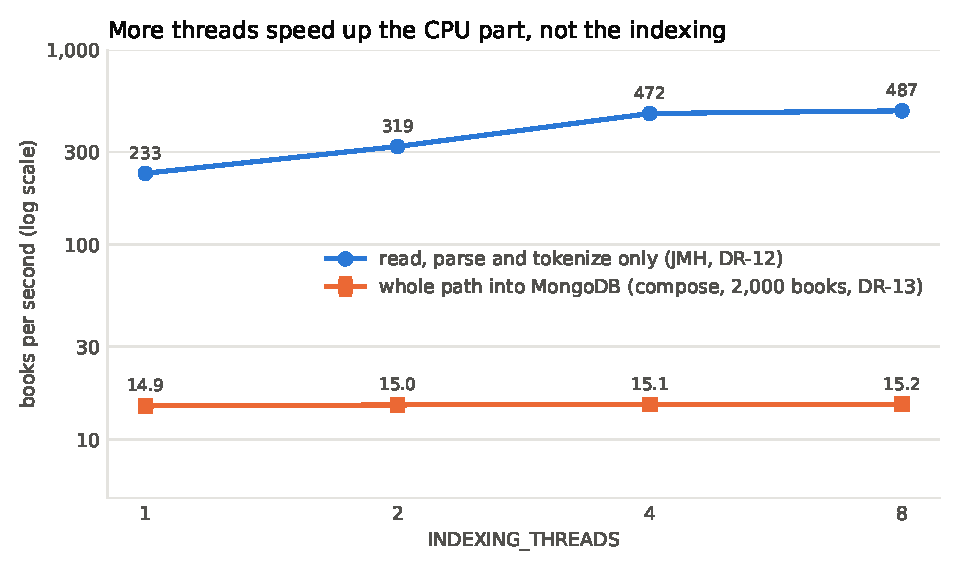
\includegraphics[width=0.49\linewidth]{figures/index_threads.pdf}\hfill
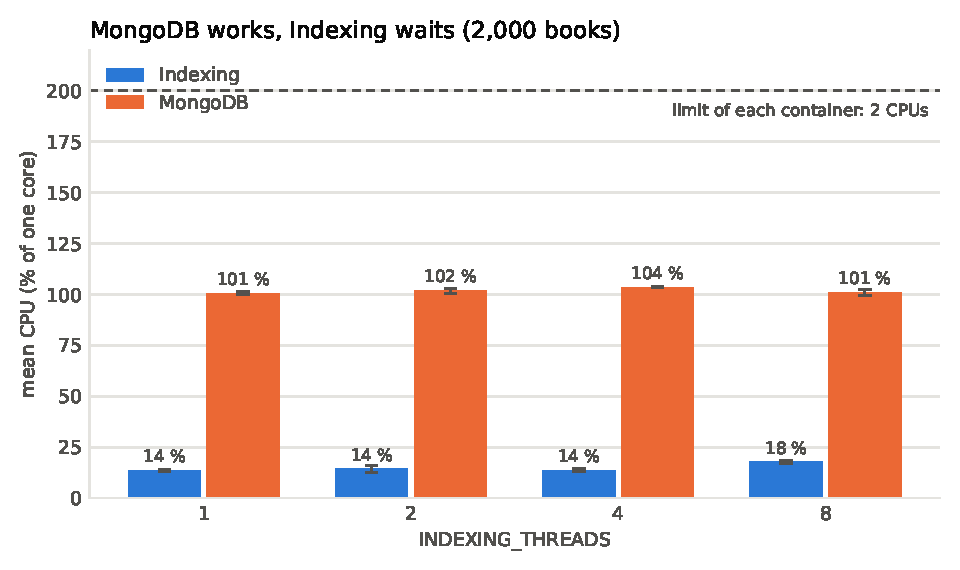
\includegraphics[width=0.49\linewidth]{figures/index_threads_cpu.pdf}
\caption{Left: books per second against the parser threads, for the CPU part alone (JMH) and for the whole path into
MongoDB. Right: mean CPU of Indexing and MongoDB in those runs.}
\label{fig:index-threads}
\end{figure}

\textbf{Scale.} 4 threads, 1 replica; 30,000 books ran once because one run takes more than 4~hours:

\begin{table}[H]
\centering\small
\begin{tabular}{@{}rrrrrrr@{}}
\toprule
\textbf{Books} & \textbf{Runs} & \textbf{Books/s} & \textbf{Duration} & \textbf{Terms} & \textbf{Index on disk} &
  \textbf{Longest list} \\
\midrule
200 & 3 & 24.90 $\pm$ 0.02 & 11 s & 58,244 & 5.8 MB & 200 ids \\
10,000 & 3 & 5.54 $\pm$ 0.01 & 30 min & 394,502 & 465 MB & 9,965 ids, 99 KB \\
30,000 & 1 & 2.00 & 4 h 10 min & 651,565 & 1.11 GB & 29,898 ids, 318 KB \\
\bottomrule
\end{tabular}
\caption{Indexing against the number of books. Peak memory: Indexing 404 to 518~MiB, MongoDB 461 to 802~MiB of its
1~GB, Hazelcast 326 to 390~MiB.}
\label{tab:index-scale}
\end{table}

\begin{figure}[H]
\centering
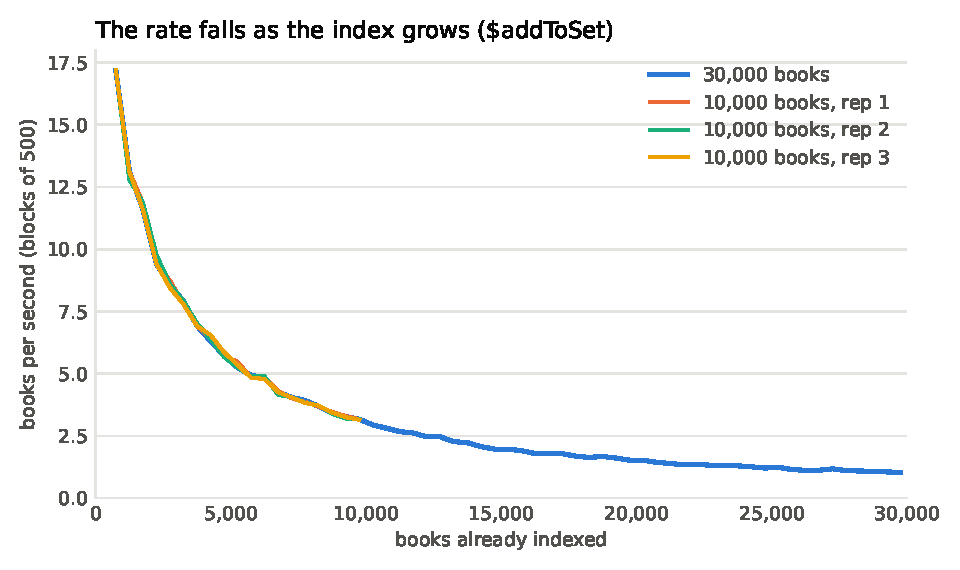
\includegraphics[width=0.75\linewidth]{figures/index_rate.pdf}
\caption{Books per second against the books already in the index, in blocks of 500 books (5 batches). The three runs
of 10,000 books and the run of 30,000 lie on one curve.}
\label{fig:index-rate}
\end{figure}

\textbf{Probe of the posting lists.} To isolate the cost of one update, the driver adds 100 ids to a single posting
list of a given length, 20 times, with \code{\$addToSet} and with \code{\$push}:

\begin{figure}[H]
\centering
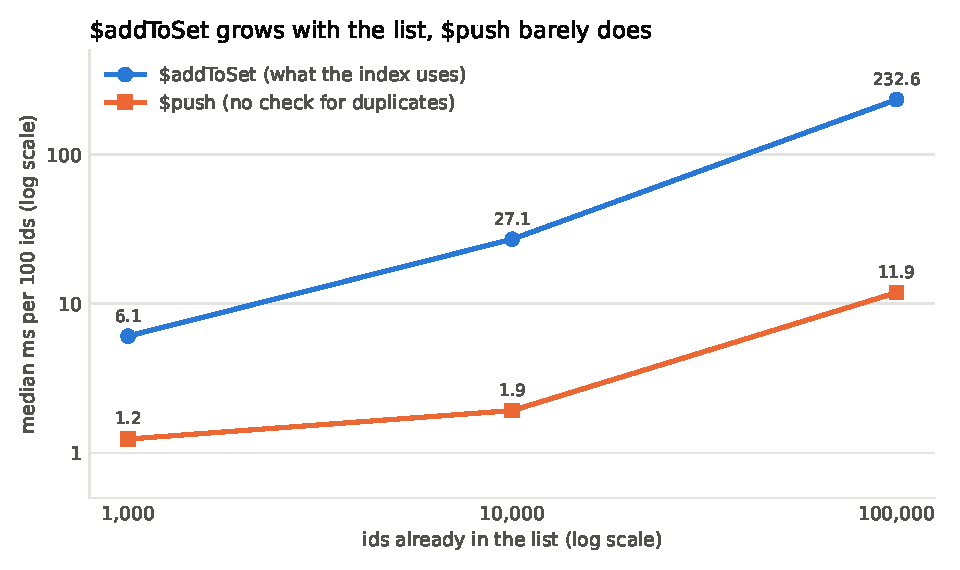
\includegraphics[width=0.49\linewidth]{figures/index_probe.pdf}\hfill
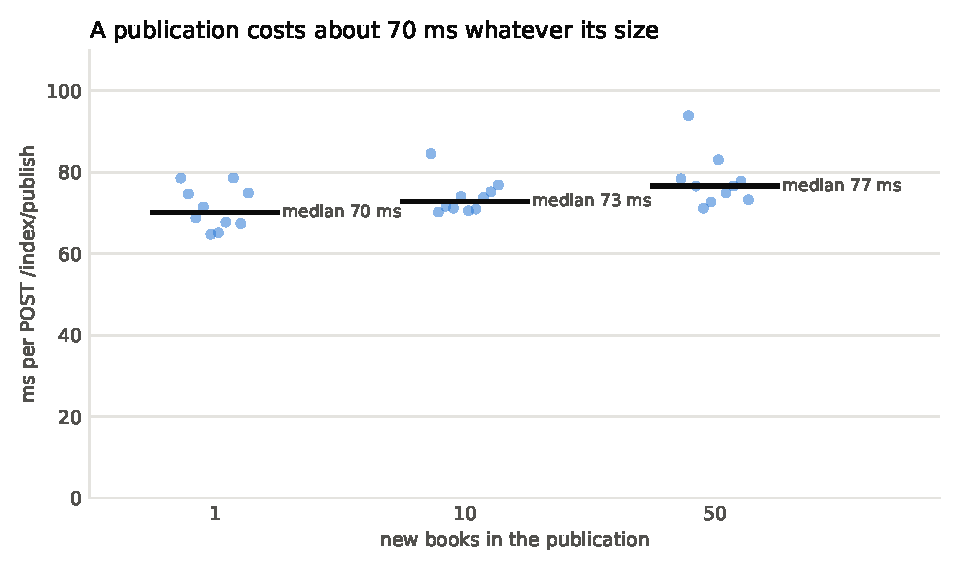
\includegraphics[width=0.49\linewidth]{figures/index_publish.pdf}
\caption{Left: median time to add 100 ids to one posting list. Right: each \code{POST /index/publish} of 1, 10 and 50
new books on an index of 10,000 books, 10 times each, and the median.}
\label{fig:index-probe-publish}
\end{figure}

\textbf{Publication.} \code{POST /index/publish} on an index of 10,000 books takes a median of 70, 73 and 77~ms for 1, 10
and 50 new books (Figure~\ref{fig:index-probe-publish}). The first publication, with all 10,000 books, took 459~ms.

\subsection{Analysis}

\begin{itemize}
  \item \textbf{Indexing is limited by MongoDB, not by its own CPU.} From 1 to 8 threads the rate improves by 2~\%,
        within the noise, while the CPU part alone doubles. Indexing uses less than a fifth of one core. MongoDB uses
        about one core of its two for the whole run, because a single writer sends one bulk write at a time: the work
        of MongoDB is one serial stream.
  \item \textbf{The rate falls as the index grows, and \code{\$addToSet} explains it.} At 10,000 books a batch of 100
        takes about 33~s, at 30,000 about 90~s. The probe shows why: \code{\$addToSet} compares each new id with the
        whole list, so its cost grows linearly with the list, 14 times that of \code{\$push} at 10,000 ids and 20 times
        at 100,000. The frequent terms hold almost one id per book, so every batch pays for the size of the index.
        The two scales agree where they overlap: books 9,000 to 12,000 of the 30,000 run went at 2.9 books/s, and the
        last tenth of the 10,000 runs at 3.2.
  \item \textbf{Publishing is cheap and its cost is fixed.} From 1 to 50 new books the median grows by 7~ms: the round
        trips of its steps dominate, not the books. The Control can therefore publish often, every 30~s or every 100
        books, without loading MongoDB.
  \item \textbf{Saturation point.} On this host and these limits, indexing does not saturate a resource of its own: it
        is bound by the time MongoDB takes per update, which grows with the index. Adding threads or replicas to
        Indexing changes nothing; changing the write (Section~\ref{sec:decisions-storage}) or giving MongoDB more cache
        and CPU would.
\end{itemize}

\textbf{Limits of these measures.}
\begin{itemize}
  \item Everything runs on one machine: the driver, \code{docker stats} and the services share its CPUs.
  \item The WiredTiger cache (0.25~GB) is smaller than the index from 10,000 books on. The probe isolates
        \code{\$addToSet} on one document, but in the full runs part of the slowdown may also come from the cache.
  \item MongoDB is not restarted between runs, only its database is deleted, so its peak memory grows along the run
        whatever the level.
  \item With 200 books only 1 or 2 samples of the monitor fall inside the run, so its CPU figures are not meaningful.
  \item 100,000 books were not measured: even at the rate of the last books of the 30,000 run, about one book per
        second and still falling, the 70,000 more books would take over 19~hours.
  \item Indexing replicas were not measured for throughput: by design only one writes. Their failover was measured
        (Section~\ref{sec:indexing}).
\end{itemize}

\section{Benchmarks and results: Search}
\label{sec:benchmarks}

This part covers Search; Section~7 of the final report consolidates it with the other services. The scripts and
the instructions to repeat every measure are in \code{benchmarks/search/}.

\subsection{Reference machine}

All the valid measures come from one machine, idle during the run. \code{host.txt} records each run.

\begin{table}[H]
\centering\small
\begin{tabularx}{\linewidth}{@{}L{3.2cm}X@{}}
\toprule
CPU & Intel Core i7-9750H, 2.60 GHz: 6 cores, 12 logical CPUs \\
Memory and storage & 16 GB, NVMe SSD \\
Operating system & Ubuntu 24.04, Linux 7.0 \\
JVM & OpenJDK 21.0.12, heap fixed at 4 GB for JMH \\
Power & Plugged in, balanced energy profile \\
Code & commit \code{263fb9f} for JMH \\
\bottomrule
\end{tabularx}
\caption{Reference machine of the benchmarks.}
\end{table}

\textbf{A deviation in the JMH run.} A loop of \code{docker stats} left over from an earlier test was running during the
measures. It takes little CPU, and the errors of the results are small, but the machine was not completely idle, as
\S6.3 of the assignment asks.

\pending{Add the Docker version and the commit of the load tests from their \code{host.txt}. If JMH is measured
again without that process, replace the numbers of this section and remove the paragraph above.}

\subsection{Microbenchmarks with JMH}

The JMH classes are in \code{search-service/src/test/java/.../benchmark}, so they are not part of the service jar,
and they run directly on the host. They measure \code{SearchEngine} on a synthetic index held in memory, without
MongoDB or HTTP, with 200, 10,000 and 100,000 books. Each configuration runs 5 warm-up and 10 measurement iterations
of 1~s in 2 separate JVMs with a fixed heap of 4~GB, and each scenario compares its result with an independent
calculation before measuring.

\begin{table}[H]
\centering\small
\begin{tabularx}{\linewidth}{@{}L{3.6cm}X@{}}
\toprule
\textbf{Benchmark} & \textbf{What changes} \\
\midrule
Intersection & Number of books and of terms in the query \\
Filters & Number of books and which filter \\
Pagination & Number of books, position of the page (0, 50 and 99 \%) and its size (20 and 100) \\
Threads & 1, 2, 4 and 8 threads on the same intersection, with 100,000 books \\
\bottomrule
\end{tabularx}
\caption{JMH experiments.}
\end{table}

\textbf{Limitation.} Each term is assigned to books at random and independently, while real words tend to appear
together. These results compare the cost of each step; they do not predict the response time of real queries.

In the synthetic index, \code{common} is in 50~\% of the books, \code{frequent} in 30~\%, \code{medium} in 10~\%
and \code{rare} in 1~\%, so the number of matches of each query is known in advance. Every value below is the
mean time of one search, with its 99.9~\% error in the CSV files.

\begin{table}[H]
\centering\small
\begin{tabularx}{\linewidth}{@{}Xrrrr@{}}
\toprule
\textbf{Query} & \textbf{Matches} & \textbf{200 books} & \textbf{10,000} & \textbf{100,000} \\
\midrule
\code{common} & 50 \% & 2.7 µs & 362 µs & 6.06 ms \\
\code{common frequent} & 15 \% & 1.5 µs & 288 µs & 3.45 ms \\
\code{common frequent medium} & 1.5 \% & 0.8 µs & 78 µs & 0.85 ms \\
\code{common rare} & 0.5 \% & 0.3 µs & 4.3 µs & 0.15 ms \\
\bottomrule
\end{tabularx}
\caption{JMH: intersection without filters, first page of 20, one thread.}
\end{table}

\begin{figure}[H]
\centering
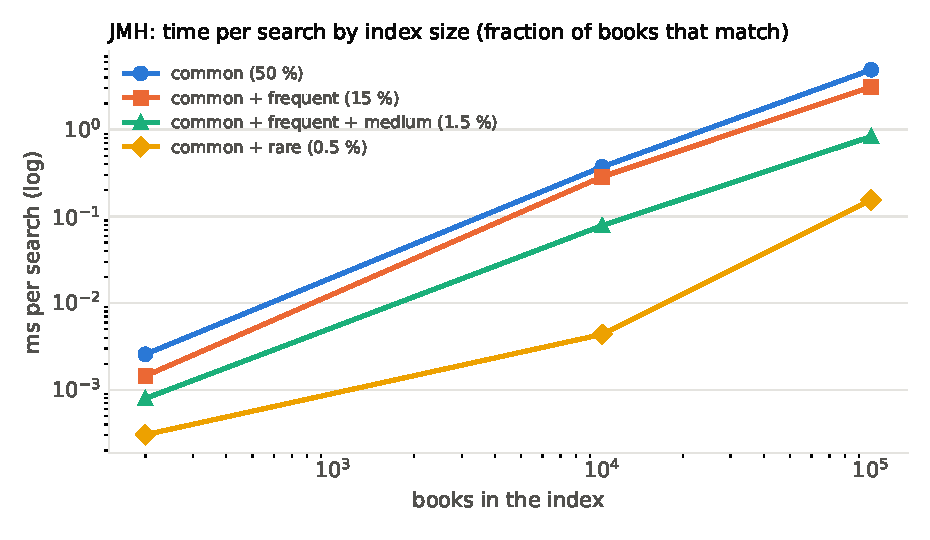
\includegraphics[width=0.82\linewidth]{figures/jmh_intersection.pdf}
\caption{Time per search against the size of the index, both axes logarithmic.}
\end{figure}

\textbf{What the intersection shows.}
\begin{itemize}
  \item \textbf{The cost follows the number of matches, not only the length of the lists.} With 100,000 books the
        four queries all read the list of \code{common}, 50,000 ids, yet they range from 6.06~ms to 0.15~ms. A rarer
        term makes the shortest list shorter, so the intersection walks fewer ids, and fewer matches are then checked
        against the snapshot, filtered and sorted.
  \item \textbf{Ten times more books cost more than ten times as much at the top of the scale.} From 10,000 to
        100,000 books, \code{common} goes from 362~µs to 6.06~ms, 16.7 times. Sorting every match grows faster than
        linearly, and the larger lists no longer fit in the CPU caches. These are our explanations; they were not
        measured separately.
\end{itemize}

\textbf{Filters.} With 100,000 books and the query \code{common}, no filter takes 4.97~ms. The language filter adds
5~\% and the author filter 12~\%, because it compares strings ignoring case; all of them together, 14~\%. The year
filter takes 8~\% less, because it leaves fewer books to sort. Filters run in memory on the metadata of the snapshot,
after the intersection, so they never add a query to MongoDB.

\textbf{Pagination.} The position of the page does not change the cost: with 100,000 books, the first page, the middle
one and one near the end all take about 4.84--4.87~ms, within the error, and so do pages of 100 results. Every search
does all the work (intersection, filters, ordering of every match) before cutting the page, and the cut itself costs
almost nothing. The other side is that the first page is not cheaper either: a user who only looks at 20 results
pays for all of them. Caching the result of a query until the next version is published would avoid it, because a
snapshot never changes.

\begin{figure}[H]
\centering
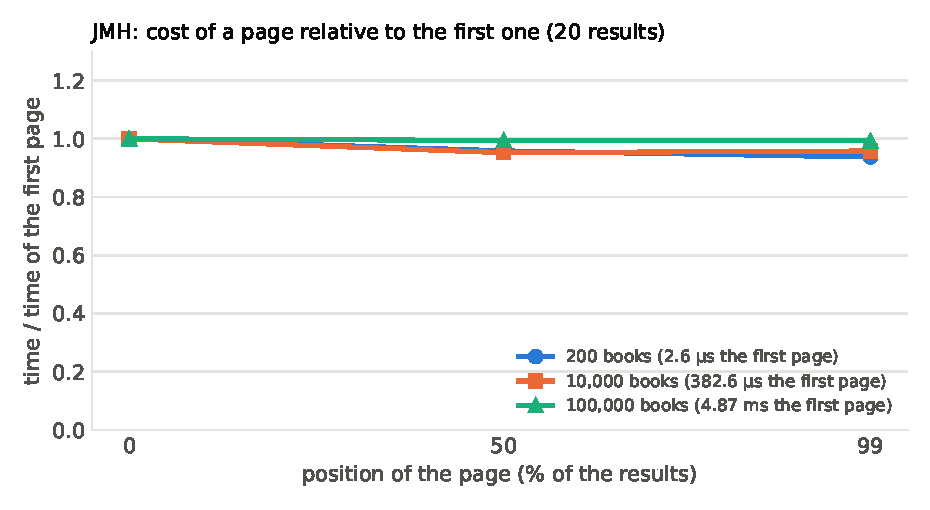
\includegraphics[width=0.82\linewidth]{figures/jmh_pagination.pdf}
\caption{Time of a page relative to the first page, pages of 20 results.}
\end{figure}

\textbf{Threads.} \code{SearchEngine} has no state of its own and the snapshot is immutable, so several threads
search at once without locks. With 100,000 books and \code{common frequent}, 2 threads complete 1.9 times as many
searches per second as one, 4 threads 3.6 times and 8 threads 5.7 times. Each search becomes slower as threads are
added, from 3.31~ms with one to 4.62~ms with eight. The threads do not wait for each other, but they share the CPU
caches and the memory bandwidth, and 8 threads exceed the 6 physical cores of the machine.

\begin{figure}[H]
\centering
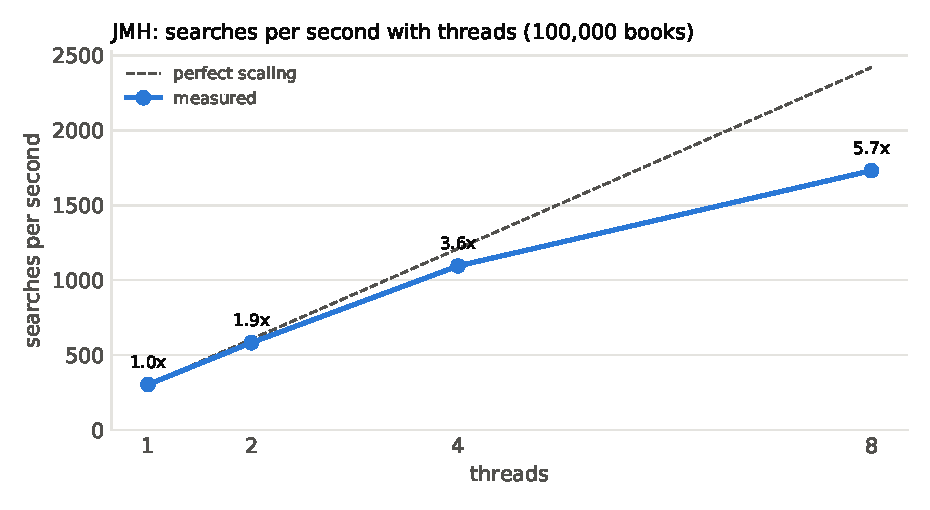
\includegraphics[width=0.82\linewidth]{figures/jmh_threads.pdf}
\caption{Searches per second with 1 to 8 threads, against perfect scaling.}
\end{figure}

This is the cost of the code alone. A real search adds MongoDB, which returns the posting lists, HTTP and nginx: the
load tests measure them.

\subsection{Load tests}

\code{LoadGenerator} sends \code{GET /search} through nginx with \code{shared/queries.txt}, and checks each answer
against the total and version it obtained first: more replicas must not change the results. Before measuring, the
script runs \code{validate-api.sh}. Each configuration is repeated 3 times with 15~s of warm-up and 30~s of measure,
and one factor changes at a time:

\begin{table}[H]
\centering\small
\begin{tabularx}{\linewidth}{@{}L{1.9cm}L{5.2cm}X@{}}
\toprule
\textbf{Experiment} & \textbf{What changes} & \textbf{Fixed} \\
\midrule
Clients & 1, 8, 32, 128, 256 clients with 1, 2 and 4 replicas & 250 threads, pool of 50, nginx with 2 CPUs \\
Threads & 16 and 64 Jetty threads, with the same clients & 1 replica, pool of 50, nginx with 2 CPUs \\
Pool & 10 and 100 MongoDB connections, with 32, 128 and 256 clients & 1 replica, 250 threads, nginx with 2 CPUs \\
nginx & 0.5 CPUs, the limit of the deployment, with 32, 128 and 256 clients & 1 replica, 250 threads, pool of 50 \\
Index size & 200 real books, and 100,000 synthetic ones if available & Same as the clients experiment \\
\bottomrule
\end{tabularx}
\caption{Load experiments. Client concurrency, threads per process and replicas are kept apart.}
\end{table}

\textbf{Why nginx has 2 CPUs here.} Short trial runs showed that nginx, with the 0.5 CPUs of the deployment,
saturated before Search and hid the effect of everything else. The experiments therefore give it 2 CPUs and measure
the 0.5 limit separately.

\textbf{Limitations.}
\begin{itemize}
  \item The generator runs on the same machine as the system, so it competes with it for CPU.
  \item It is a closed loop: under saturation, clients wait instead of queuing more requests, so latencies are lower
        than with requests arriving at a fixed rate.
  \item With 4 replicas the limits of the containers add up to 14 CPUs, which may exceed the host. Then the limits no
        longer bound each container, and the replicas compete for the same cores.
\end{itemize}

\pending{Insert the tables and figures of \code{results/analysis/}: throughput and p95 against clients for each number
of replicas, the effect of threads and of the pool, and CPU and memory per container.}

\subsection{Analysis}

\pending{Write it from the measures, without assuming the outcome. It must answer: at how many clients does the
throughput stop growing, and what happens to p95 and p99? Which container reaches its CPU limit first (Search, MongoDB
or nginx)? Do replicas and threads help, and if not, why? Is the pool of 50 connections too small or too large, as this
was an estimate? Does a larger index move the bottleneck to MongoDB? Were there errors or wrong results?}

\pending{State what was not measured and why: full pipeline under load, 100,000 books if DR-16 did not arrive.}

\section{Benchmarks and results: consolidation}
\label{sec:consolidation}

This part puts the measures of the three services side by side: one host, the configurations measured, and where each
part of the system saturates.

\subsection{The host}

Every valid measure ran on one machine, recorded by the \code{host.txt} of each run:

\begin{table}[H]
\centering\small
\begin{tabularx}{\linewidth}{@{}L{3.4cm}X@{}}
\toprule
CPU & Intel Core i7-9750H, 2.60~GHz: 6 cores, 12 logical CPUs \\
Memory and storage & 16~GB; NVMe SSD \\
Operating system & Ubuntu 24.04.5, Linux 7.0 \\
Docker & 28.3.3, sees the 12 CPUs and 16~GB \\
JVM & OpenJDK 21.0.12 for JMH and the drivers; the images run Java 17 \\
Power & Plugged in, balanced energy profile \\
\bottomrule
\end{tabularx}
\caption{Reference machine of all the benchmarks.}
\label{tab:host}
\end{table}

The deployment limits each container (\code{.env}): MongoDB 2 CPUs and 1~GB with a 0.25~GB cache; Indexing 2 CPUs and
1~GB; Search 2 CPUs per replica; Ingestion 1 CPU and 512~MB; each Hazelcast member 1 CPU and 768~MB; the Control and
nginx 0.5 CPUs. The load experiments of Search give nginx 2 CPUs, so that it does not hide the rest, and measure its
0.5 CPUs apart. The limits together exceed the 12 CPUs of the host only in the Search experiments with 4 replicas
(14 CPUs), where the replicas compete for the same cores.

\subsection{What was measured}

\begin{table}[H]
\centering\small
\begin{tabularx}{\linewidth}{@{}L{3.1cm}L{2.2cm}L{2.2cm}X@{}}
\toprule
\textbf{Experiment} & \textbf{Scope} & \textbf{Replicas} & \textbf{Threads and clients} \\
\midrule
Ingestion JMH & component, host & -- & 1, 2, 4, 8 workers \\
Indexing JMH & component, host & -- & 1, 2, 4, 8 parser threads \\
Search JMH & component, host & -- & 1, 2, 4, 8 threads \\
Indexing, threads & Indexing + MongoDB + Hazelcast, Docker & 1 Indexing & 1, 2, 4, 8 parser threads; 2,000 books \\
Indexing, scale & same & 1 Indexing & 4 threads; 200, 10,000, 30,000 books \\
Indexing, publication & same & 1 Indexing & 1, 10, 50 new books on 10,000 \\
Search, load & Search + MongoDB + nginx, Docker & 1, 2, 4 Search & 1 to 256 closed-loop clients; 250 Jetty threads
  (also 16 and 64); pool of 50 (also 10 and 100); nginx with 2 CPUs (also 0.5); index of 15, 197 and 10,000 books \\
Search with the pipeline & complete pipeline, Docker & 1 of each & 32 and 128 clients on 2,000 books while the
  pipeline processes new ones \\
\bottomrule
\end{tabularx}
\caption{The experiments, each labelled with what it measures. Every configuration was repeated 3 times, except the
30,000 books of Indexing (once). Client concurrency, replicas and threads are kept apart.}
\label{tab:experiments}
\end{table}

\subsection{Bottlenecks and scaling trends}

\begin{table}[H]
\centering\small
\begin{tabularx}{\linewidth}{@{}L{1.9cm}L{4.4cm}X@{}}
\toprule
\textbf{Service} & \textbf{Measured rate} & \textbf{What limits it} \\
\midrule
Ingestion & 473 $\mu$s per book with 1 worker, 155 with 8 (local source, JMH) &
  The coordination: claim and complete cost 1.6~ms per book with 1 thread and 0.36 with 8, more than the ingestion
  itself. With Project Gutenberg the download is far longer than both. \\
Indexing & 15 books/s on 2,000 books; 5.5 on 10,000; 2.0 on 30,000 &
  MongoDB: the cost of \code{\$addToSet} grows with each posting list, and one writer sends one stream of writes.
  Threads and replicas of Indexing do not change it (Section~\ref{sec:benchmarks-indexing}). \\
Search & About 7,500 req/s on 15 books whatever the replicas; on 10,000 books 1,036 req/s with 1 replica and
  2,612 with 4 &
  On a small index MongoDB is the limit: it reaches its 2 CPUs while the replicas of Search have CPU to spare. On
  10,000 books each query matches most of the index, the CPU of Search is the limit, and replicas help: 4 give 2.5
  times the peak of one, less than 4 because the host runs out of CPU (Section~\ref{sec:benchmarks}). \\
The whole system & with the pipeline running, Search 2,600 req/s and Indexing 0.91 books/s at the same time &
  MongoDB is shared: the writes of Indexing take it from 80 to 191~\% of its 2 CPUs. Indexing drops from 2.42 to
  0.91 books/s while Search is under load, and the p95 of Search with 128 clients rises from 109 to 160~ms. \\
\bottomrule
\end{tabularx}
\caption{Where each part of the system saturates on the reference machine.}
\label{tab:bottlenecks}
\end{table}

\textbf{Threads and replicas.} Threads help where the work is CPU inside one process: the workers of Ingestion and the
parsers of Indexing in JMH, and the replicas of Search when queries are long. They do not help where the limit is a shared
resource: the queue of Hazelcast for Ingestion with small books, MongoDB for Indexing, and MongoDB again for Search
on a small index. Indexing replicas are
standbys by design, so their effect is failover, not throughput.

\textbf{What was not measured.} The full pipeline with several Ingestion replicas and Project Gutenberg as the source
(the measures use the local source, so that the network does not dominate); 100,000 books, because indexing them at the
measured rate would take most of a day; and two machines, which is Stage~3.

\end{parts}

\section{Conclusions and evolution to Stage 3}
\label{sec:stage3}

\subsection{Strengths and weaknesses of the coordination}

\textbf{Strengths.} The coordination is explicit and checked: every transition is one method of one library, atomic,
and tested against real Hazelcast members. A book never changes state before its evidence is persistent, so a crash
at any point leaves a book that is either redone or recovered; the failure tests check it end to end
(Table~\ref{tab:failure-tests}). Replicas of
Ingestion and Search are added with \code{--scale} and nothing else, because nobody addresses a replica: the workers
pull from shared queues, and nginx spreads the queries. Losing the whole Hazelcast cluster costs a recovery, not data.

\textbf{Weaknesses.} Hazelcast is in memory, so the books without evidence (\code{PENDING}, or \code{INGESTING} without
\code{\_READY}) must be sent again after the cluster is lost. The lock of the index writer has no fencing token. The
leases compare the clocks of different processes. The datalake depends on a local file system and its atomic moves. Each
book costs two transactions, and both queues are single partitions that every claim goes through.

\pending{The measured part: books per second of Ingestion with 1, 2 and 4 replicas and with 1, 2, 4 and 8 workers, the
share of coordination in the time of a book, and the queue wait (benchmarks/ingestion/results/integration/), with the
bottleneck each one shows.}

\subsection{What changes on the Stage 3 cluster}

The services keep their code; what they assume about the machine does not hold on a cluster. Table~\ref{tab:stage3}
lists each local assumption and what replaces it.

\begin{table}[H]
\centering\small
\begin{tabularx}{\linewidth}{@{}L{3.6cm}L{4.3cm}X@{}}
\toprule
\textbf{Local assumption} & \textbf{Why it breaks on a cluster} & \textbf{Stage 3} \\
\midrule
Two Hazelcast members on one host & They share its failures; a backup on the same machine protects from nothing &
  One member per machine (or embedded in the services), discovery by the platform instead of a fixed list, and backups
  placed on another machine (partition groups per host or zone) \\
\code{IMap.lock} for the single writer & In a network partition each half of the cluster can grant it (split-brain), and
  it has no fencing token & A CP \code{FencedLock} (Enterprise, three or more CP members), or a lease document in MongoDB
  taken with a conditional update whose version is the fencing token for every write; a split-brain protection quorum
  on the coordination structures \\
Leases on one clock & Clocks of different machines drift; a lease could expire early or late & NTP on every node and a
  margin above the expected skew, or the time of the member that owns the entry \\
Datalake on a local file system, \code{\_READY} after atomic moves & An atomic move exists only inside one file system;
  Indexing on another machine cannot read the folder & Shared storage (an object store such as S3 or MinIO, or HDFS): write
  the book, then the marker object; readiness is the marker object \\
Recovery lists the datalake & Listing every range folder grows with the number of books, and gets slower over the network &
  A persistent log of ready books (a MongoDB collection written with the marker), read like \code{index\_log} \\
One Control & Its absence stops leases and publications; on a cluster, nodes come and go & Two or more instances with a
  leader election (the same fenced lease as the writer); the others wait as standbys \\
Queues of one partition & Every claim of every node goes to one member & Several queues by range of ids, each taken by
  some workers, or a partitioned log with acknowledgements (Kafka) if the work grows beyond what one member serves \\
Services without authentication on \code{127.0.0.1} & On a network of machines anyone could reach the Control or
  Hazelcast & TLS and authentication on the Hazelcast clients and on the internal APIs; only the load balancer exposed \\
Docker network on one host & Containers on different machines do not share it & An overlay network or an orchestrator
  (Kubernetes, Docker Swarm) with service discovery; nginx replaced by its load balancer \\
\bottomrule
\end{tabularx}
\caption{The local assumptions of the coordination and their Stage 3 replacement.}
\label{tab:stage3}
\end{table}

\textbf{What does not change.} The contract itself: the states, the transitions, the principle that evidence comes
first, the leases and the recovery are the same on one machine and on many, and the services reach Hazelcast through the
same library. That was the reason to choose it (Table~\ref{tab:alternatives}): for Stage 3 the work is in the
configuration and in the storage, not in the services.

\textbf{Distribution of work.} On a cluster the replicas of Ingestion run on several machines and keep pulling from the
same queues, so the distribution of books needs no change. What needs measuring again is where the first bottleneck moves
once each replica has a machine of its own: the queues of Hazelcast, the shared storage, or the single index writer.
\pending{Link with the conclusion of section 7: which of these limits the single-machine measurements already show.}


\end{document}
